\section{Connection Server}
\begin{figure}[h]	
	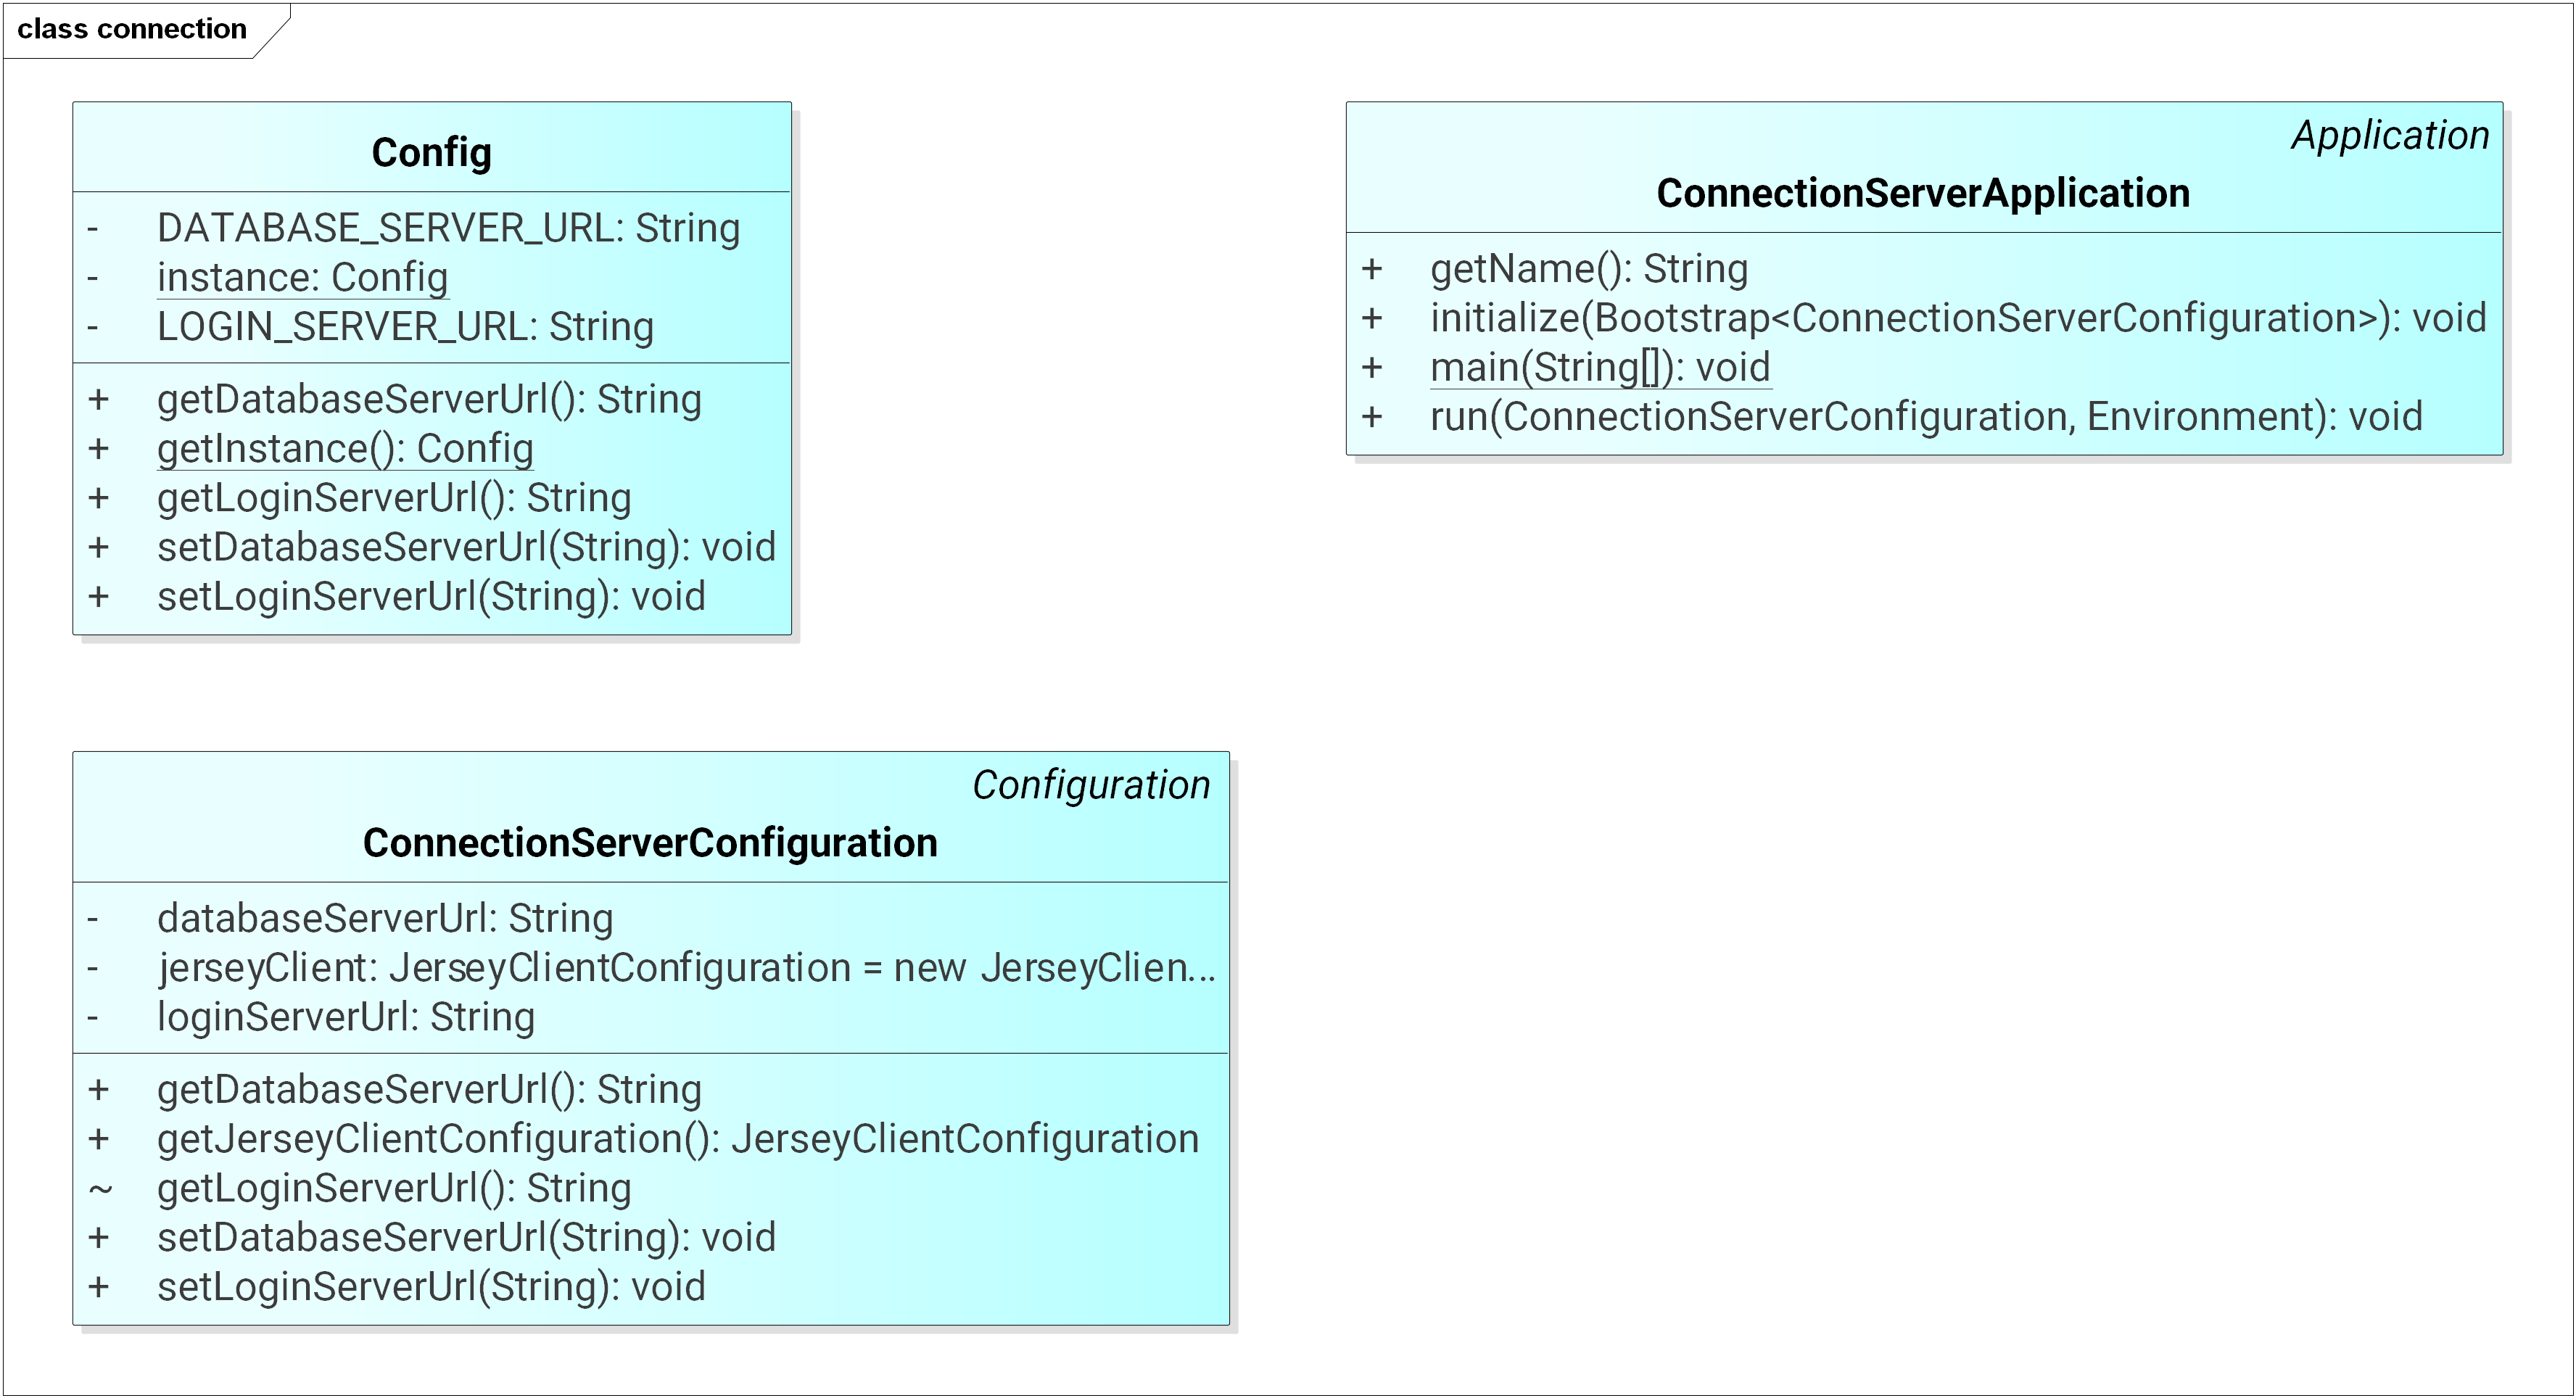
\includegraphics[width=\textwidth]{figures/classdiagrams/csconnection}
	\centering			
	\caption{Class diagram of package \textit{bachelors.connection}}
\end{figure}

\begin{figure}[h]	
	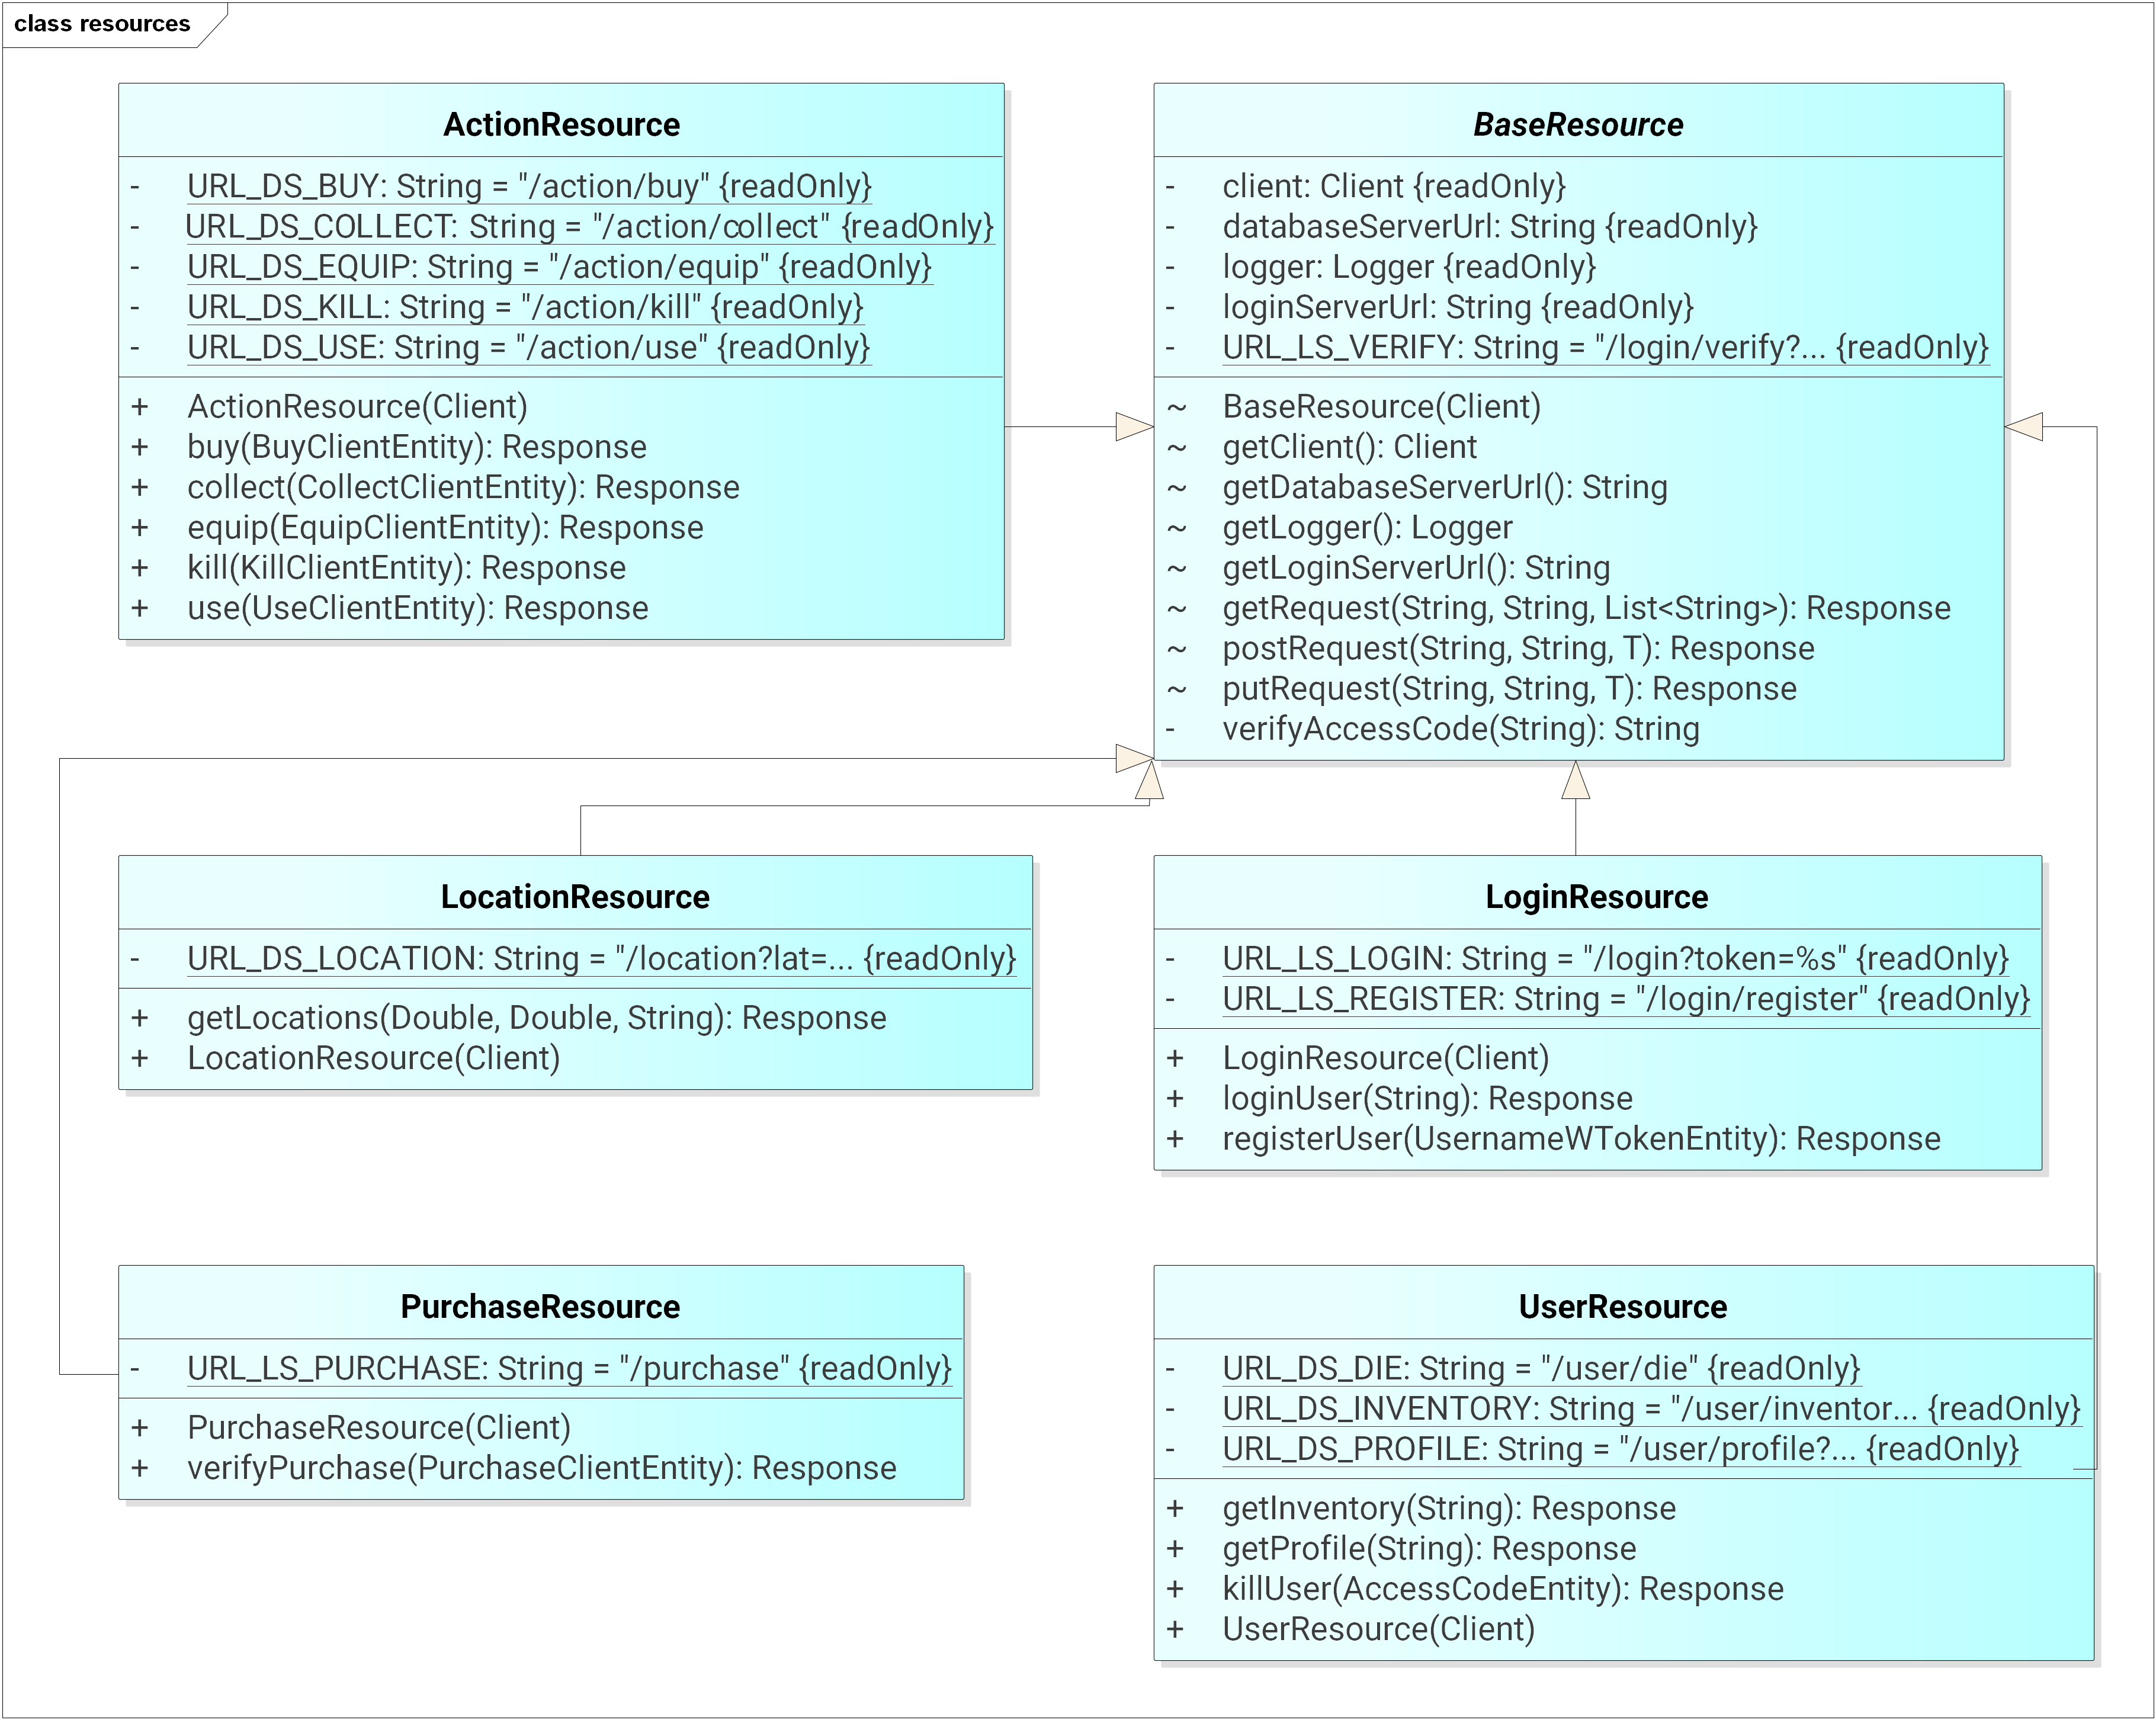
\includegraphics[width=\textwidth]{figures/classdiagrams/csresources}
	\centering			
	\caption{Class diagram of package \textit{bachelors.connection.resources}}
\end{figure}

\begin{figure}[h]	
	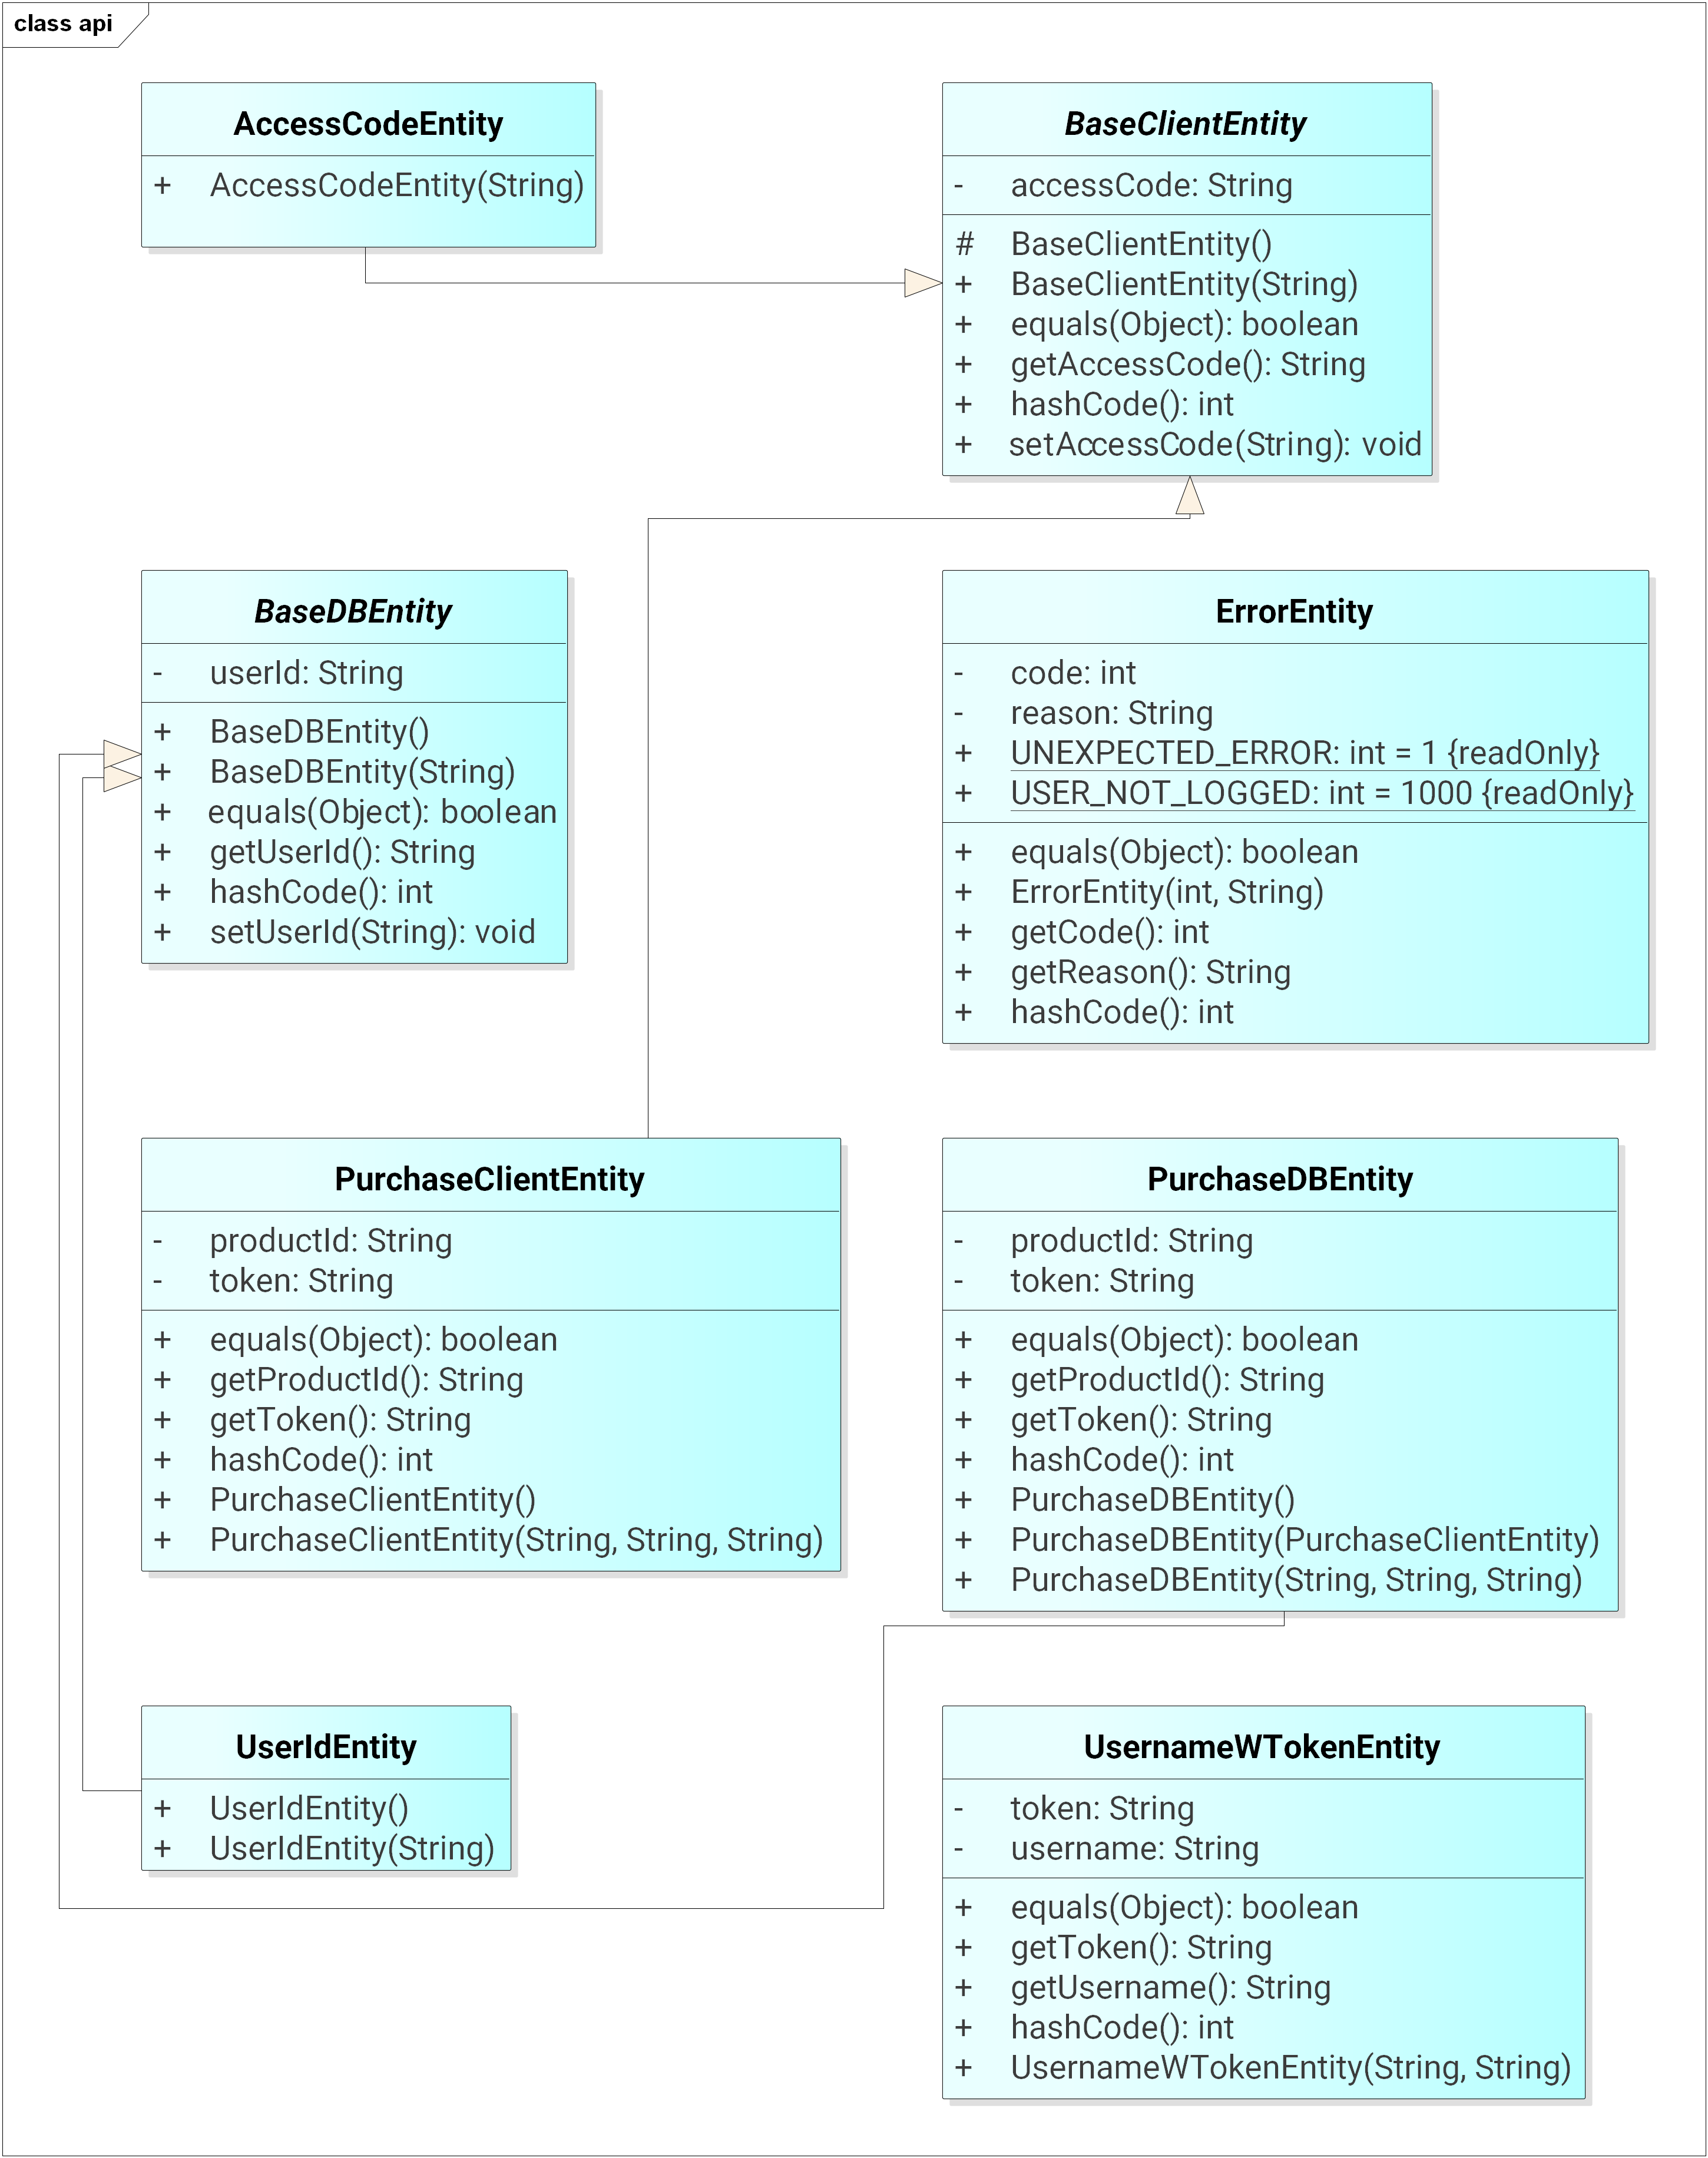
\includegraphics[width=\textwidth]{figures/classdiagrams/csapi}
	\centering			
	\caption{Class diagram of package \textit{bachelors.connection.api}}
\end{figure}

\begin{figure}[h]	
	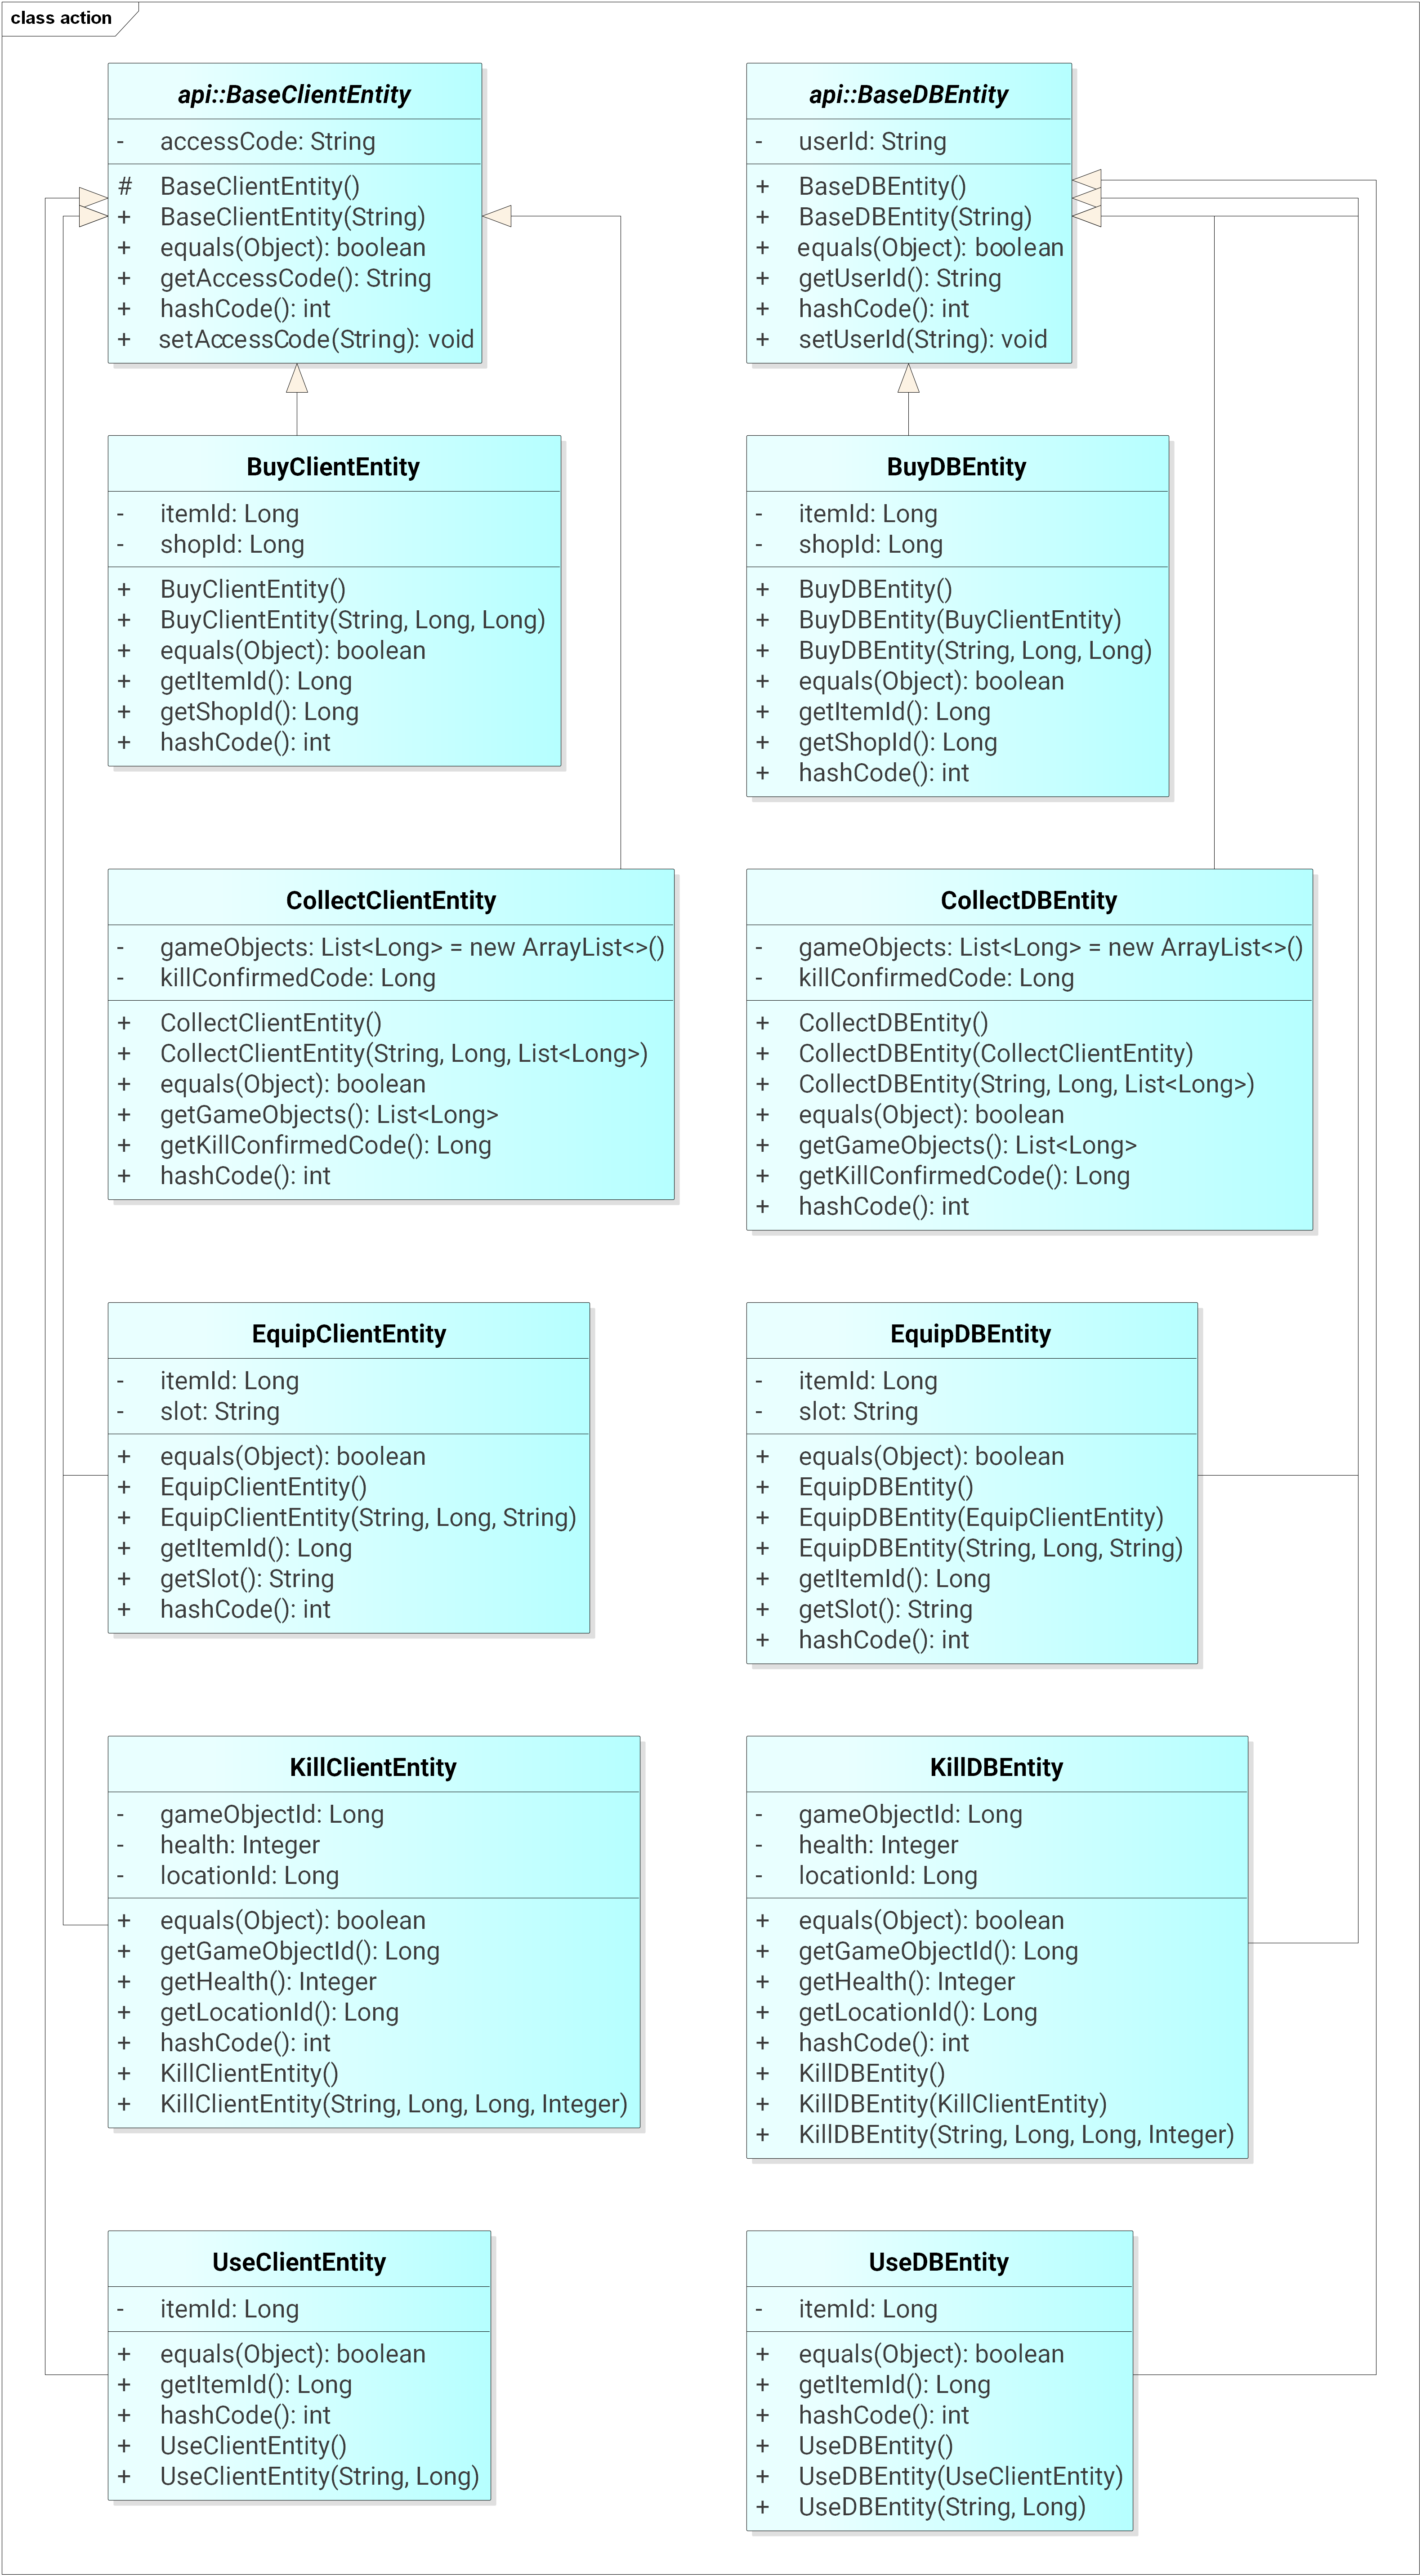
\includegraphics[height=0.9\textheight]{figures/classdiagrams/csaction}
	\centering			
	\caption{Class diagram of package \textit{bachelors.connection.api.action}}
\end{figure}




\section{Database Server}
\begin{figure}[h]	
	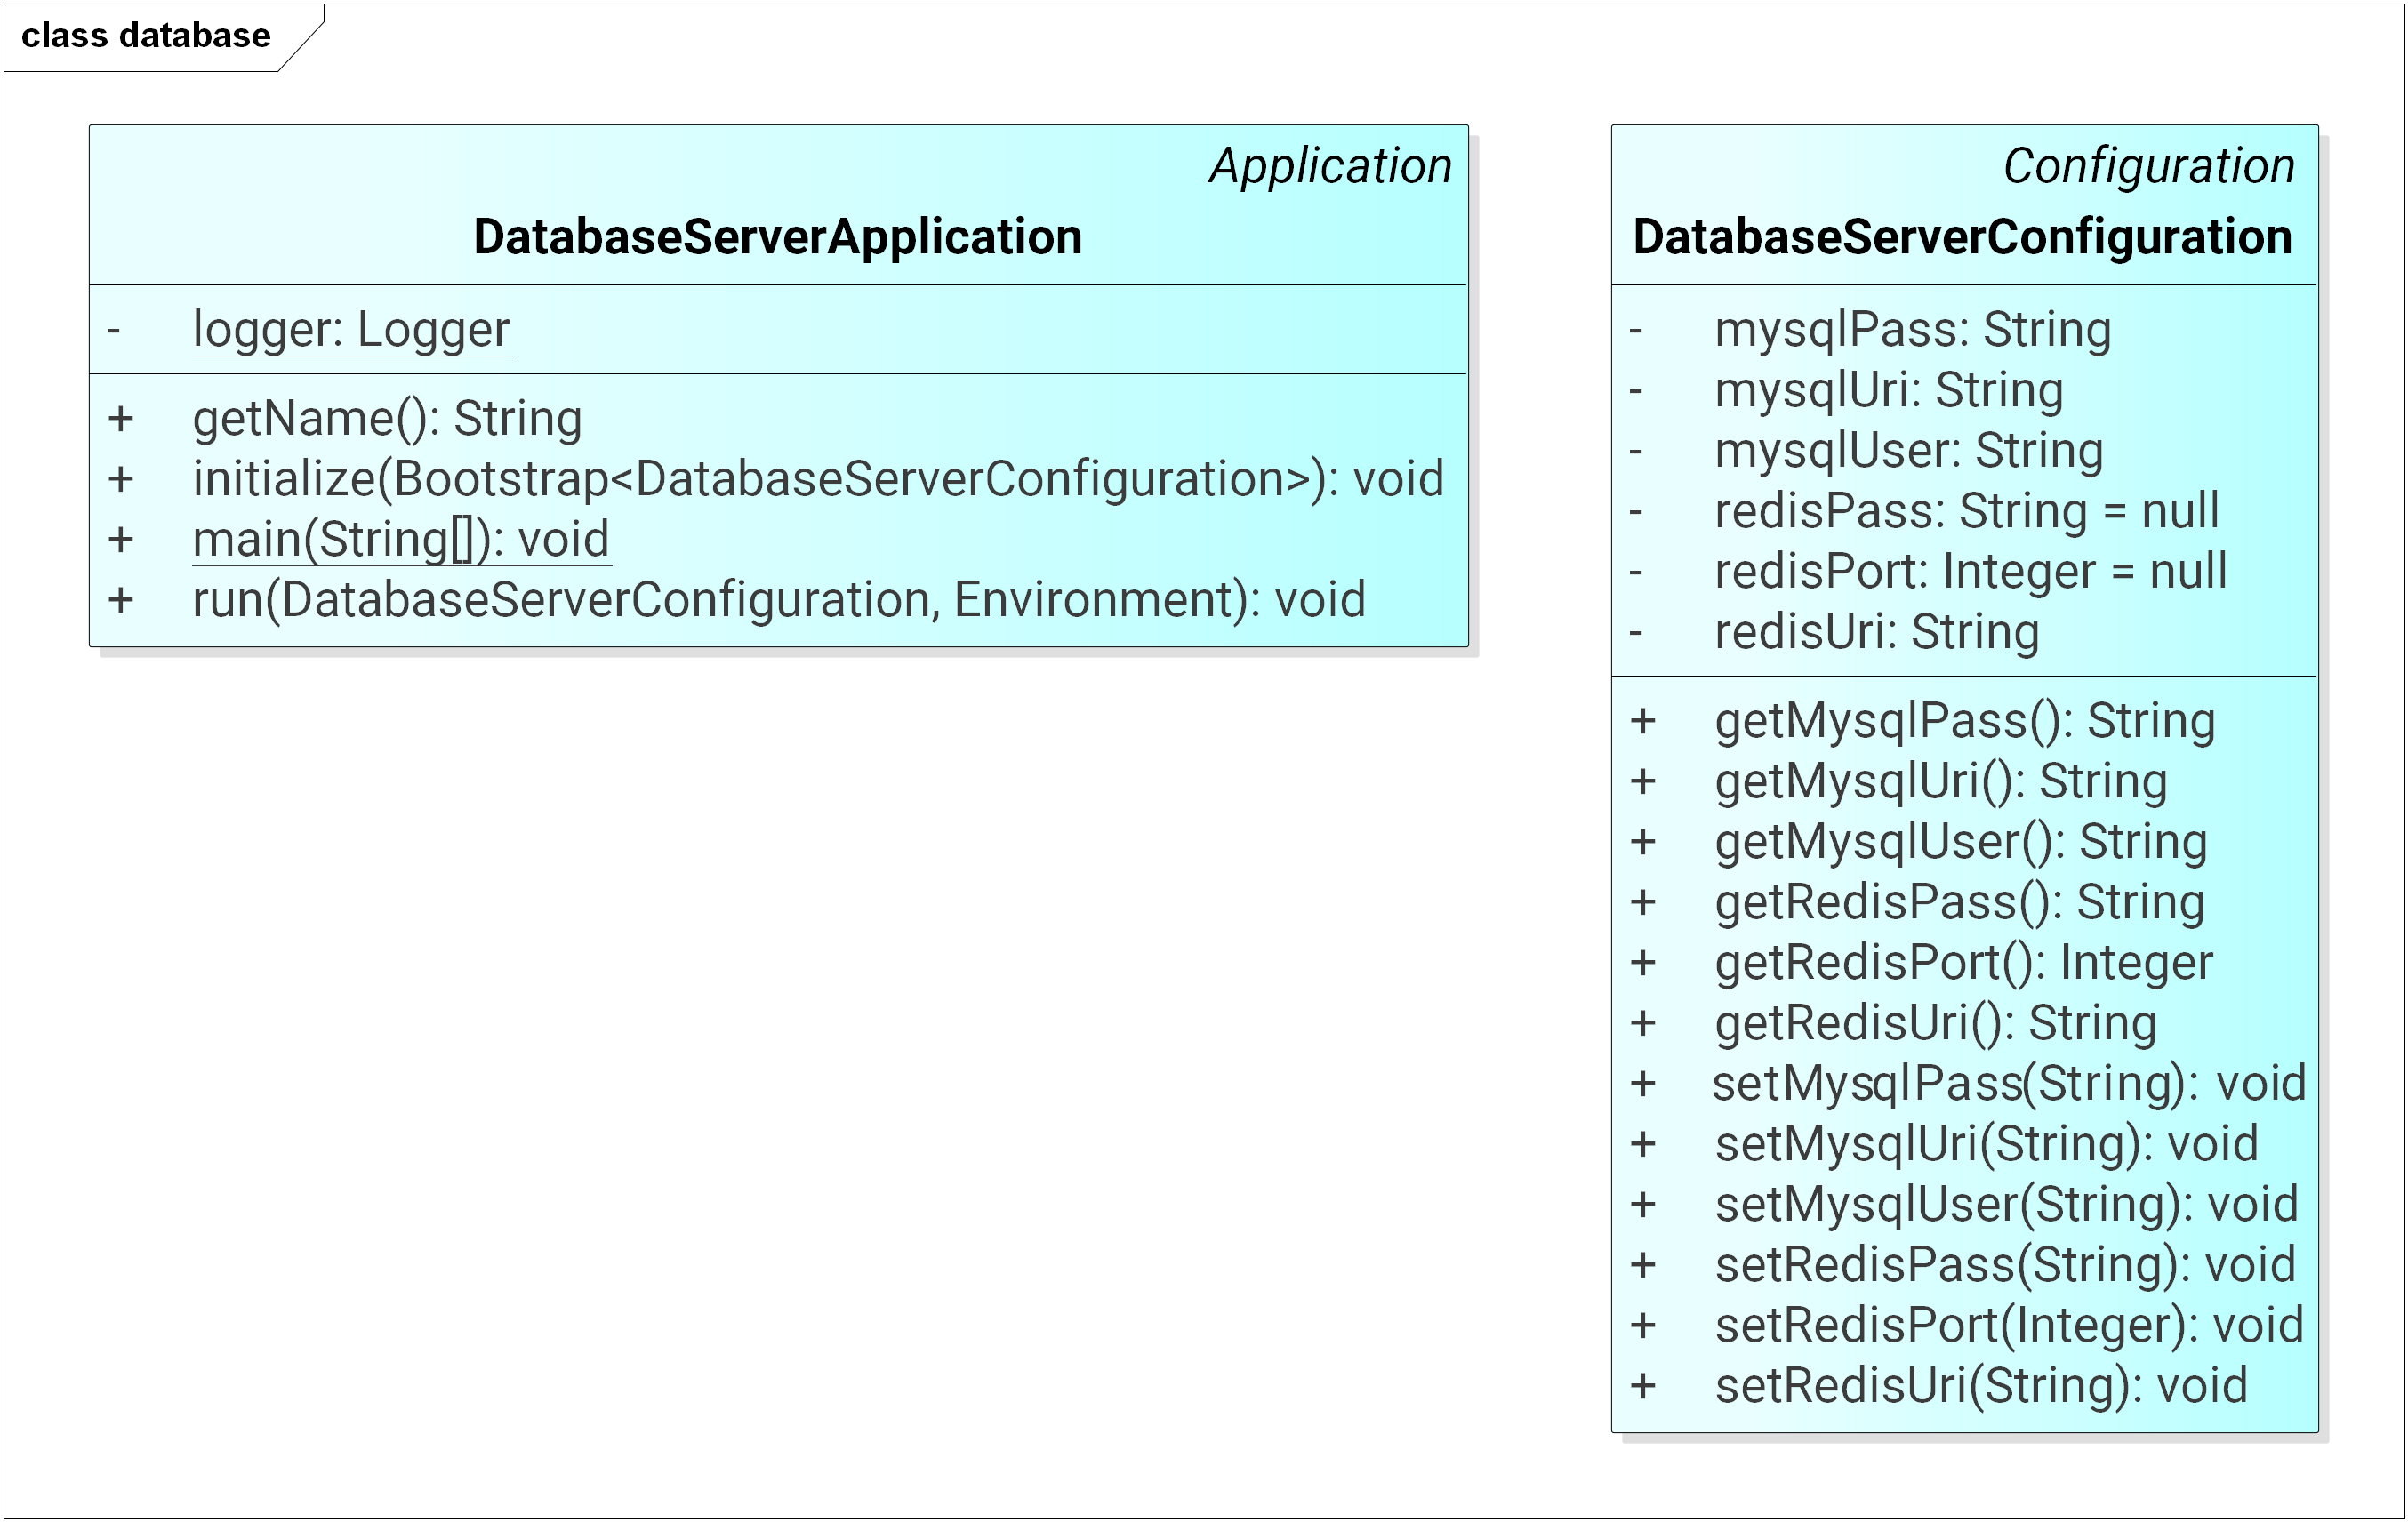
\includegraphics[width=\textwidth]{figures/classdiagrams/dsdatabase}
	\centering			
	\caption{Class diagram of package \textit{bachelors.database}}
\end{figure}

\begin{figure}[h]	
	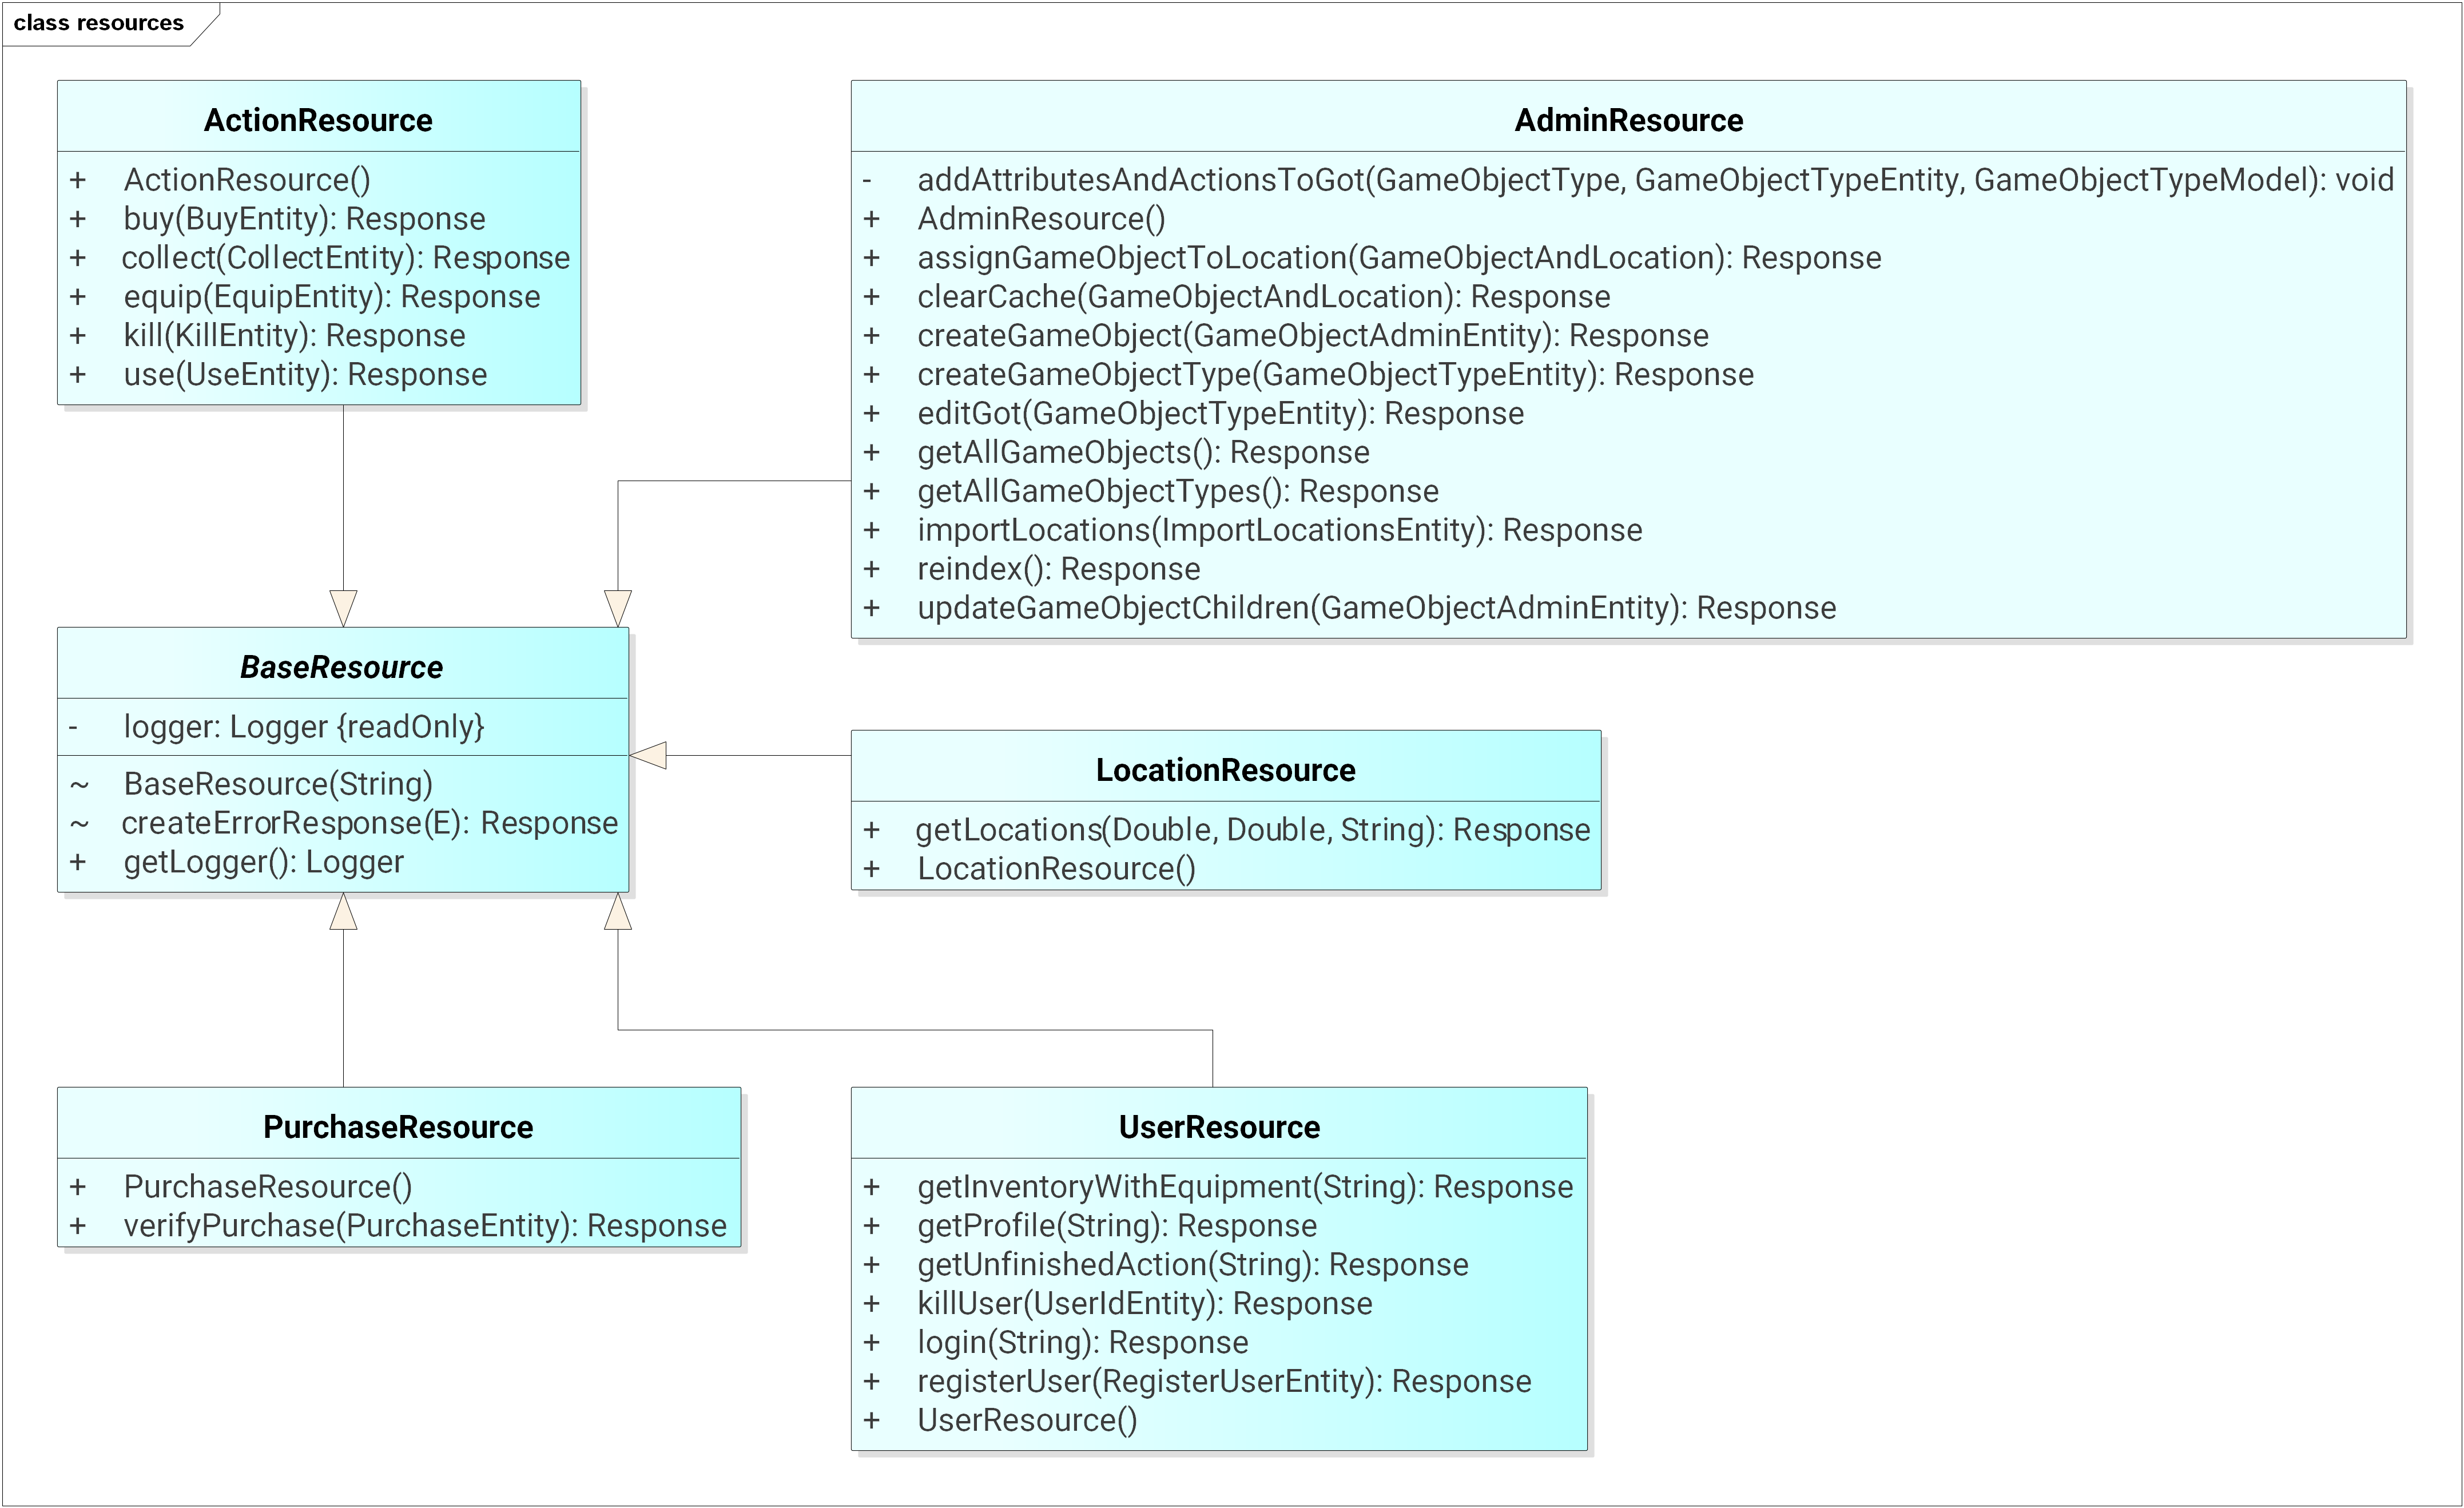
\includegraphics[width=\textwidth]{figures/classdiagrams/dsresources}
	\centering			
	\caption{Class diagram of package \textit{bachelors.database.resources}}
\end{figure}

\begin{figure}[h]	
	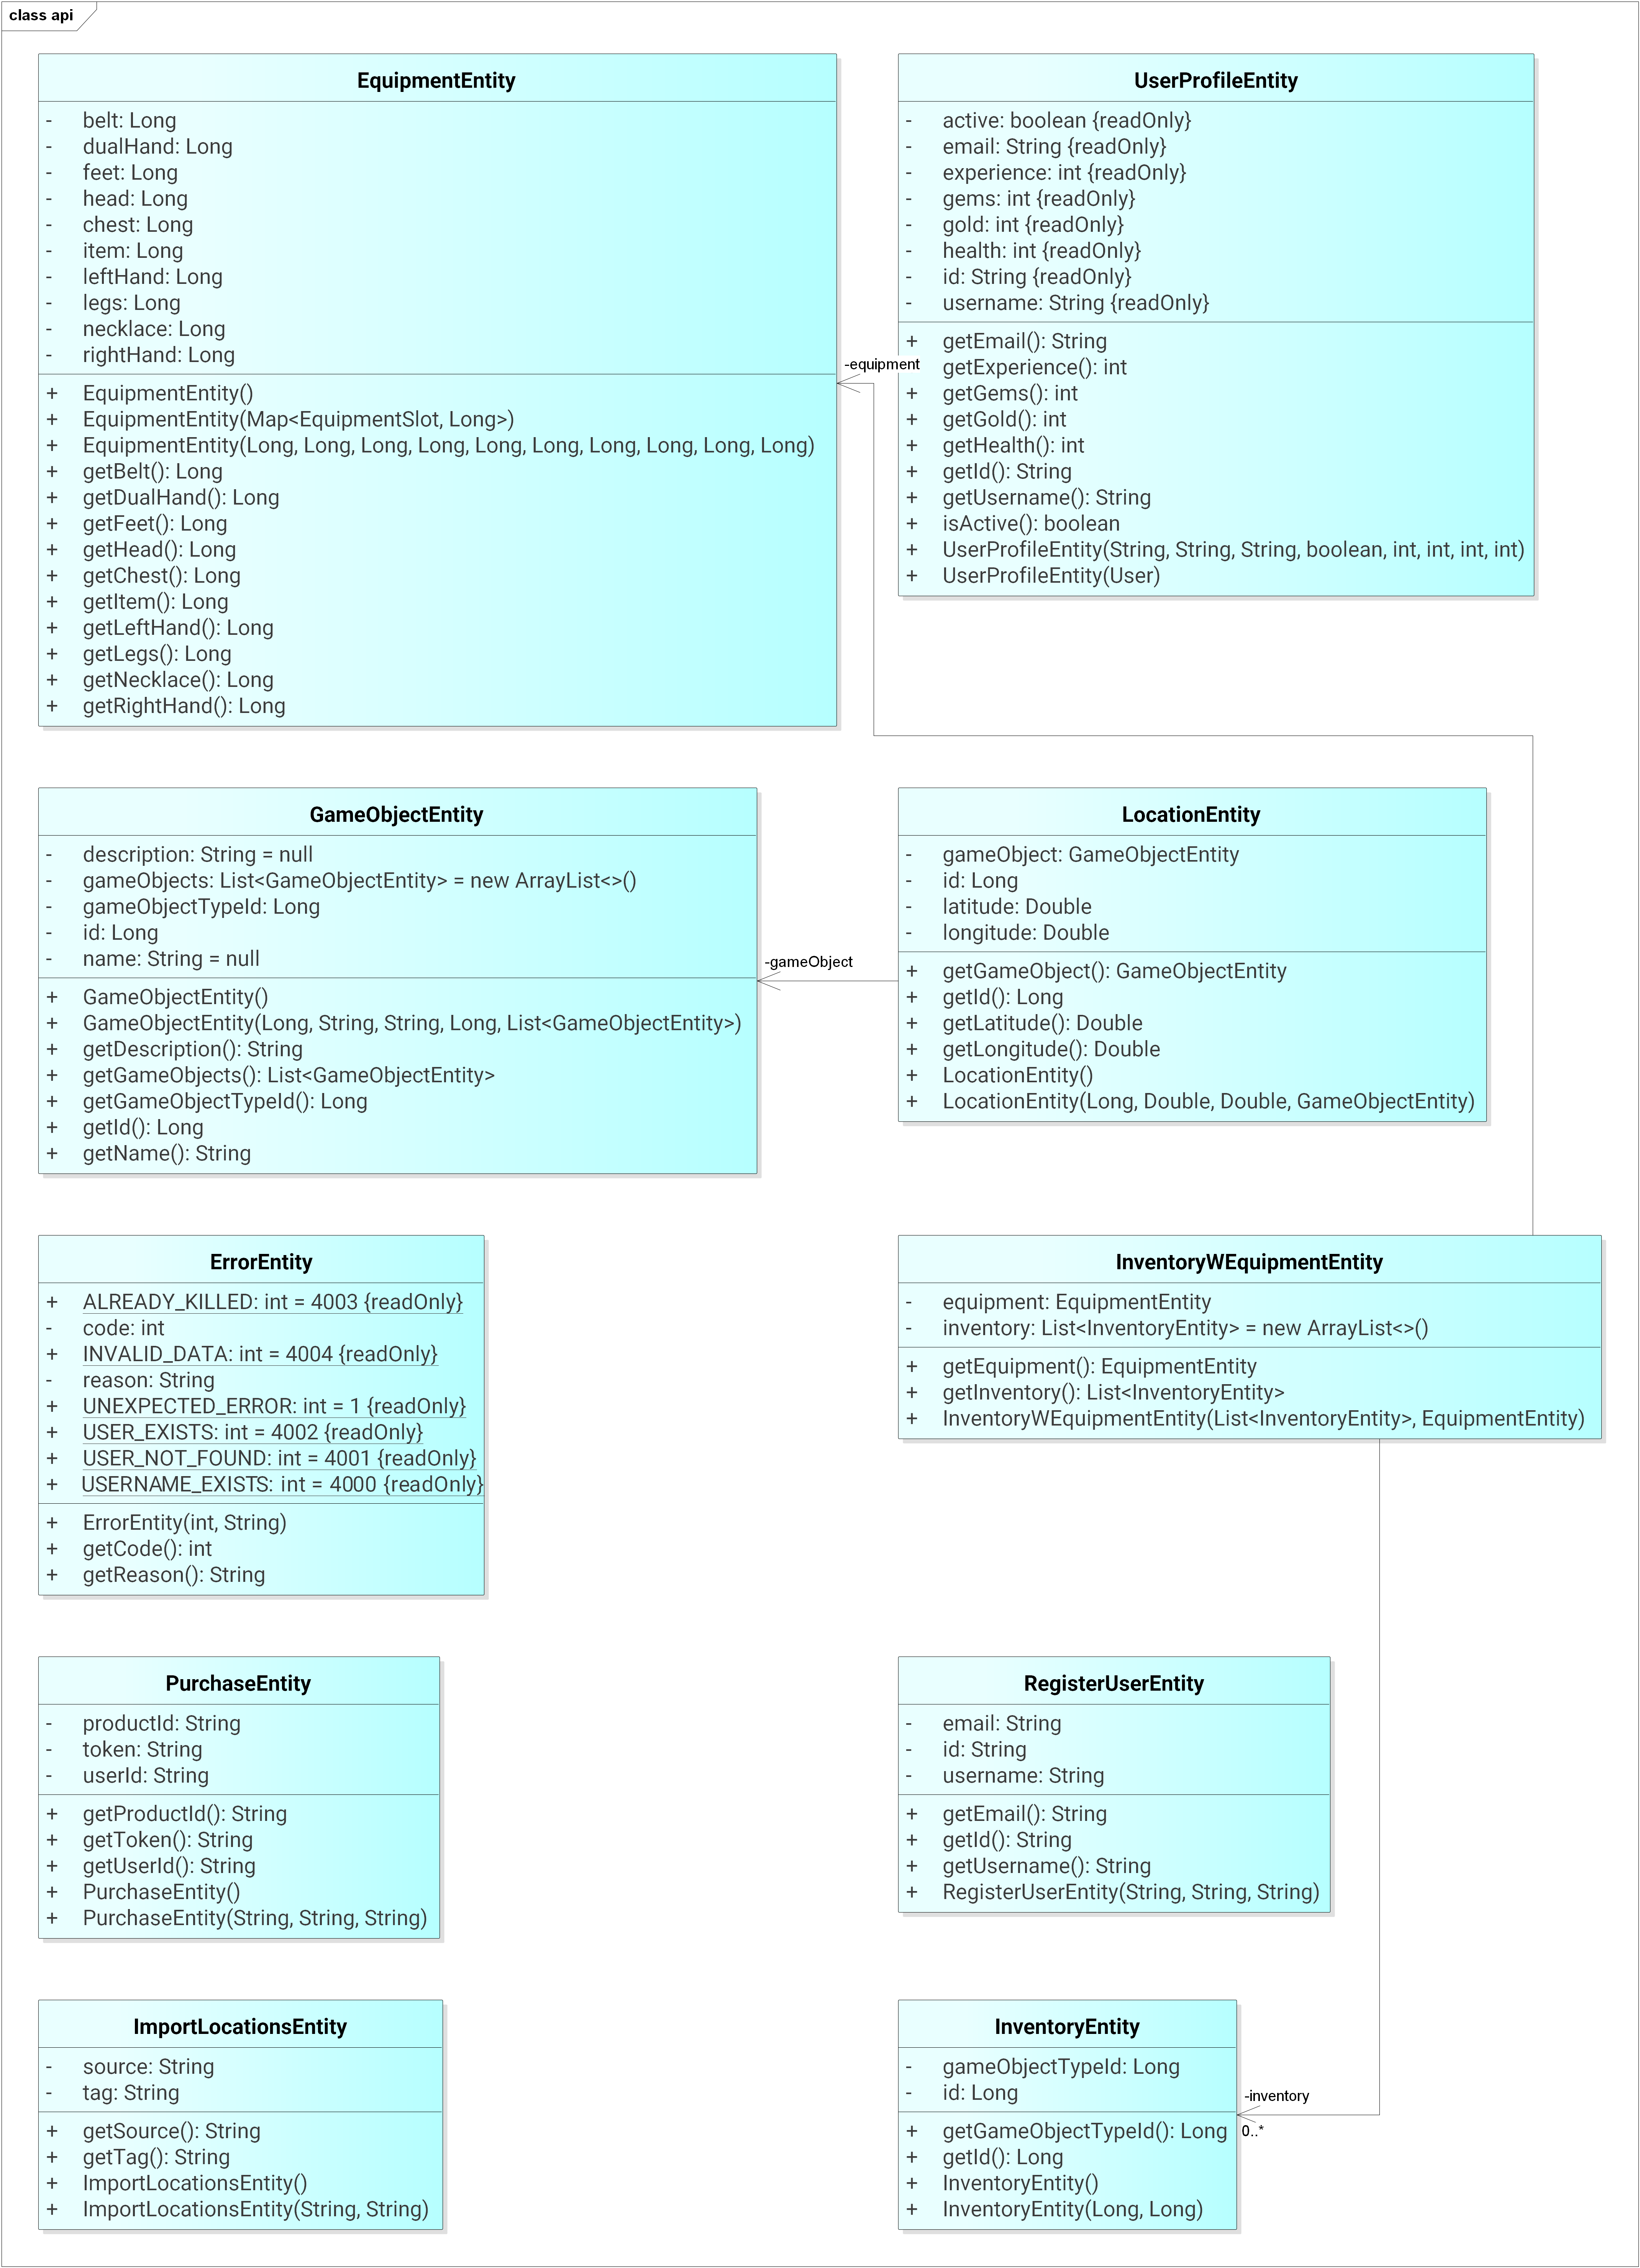
\includegraphics[width=\textwidth]{figures/classdiagrams/dsapi}
	\centering			
	\caption{Class diagram of package \textit{bachelors.database.api}}
\end{figure}

\begin{figure}[h]	
	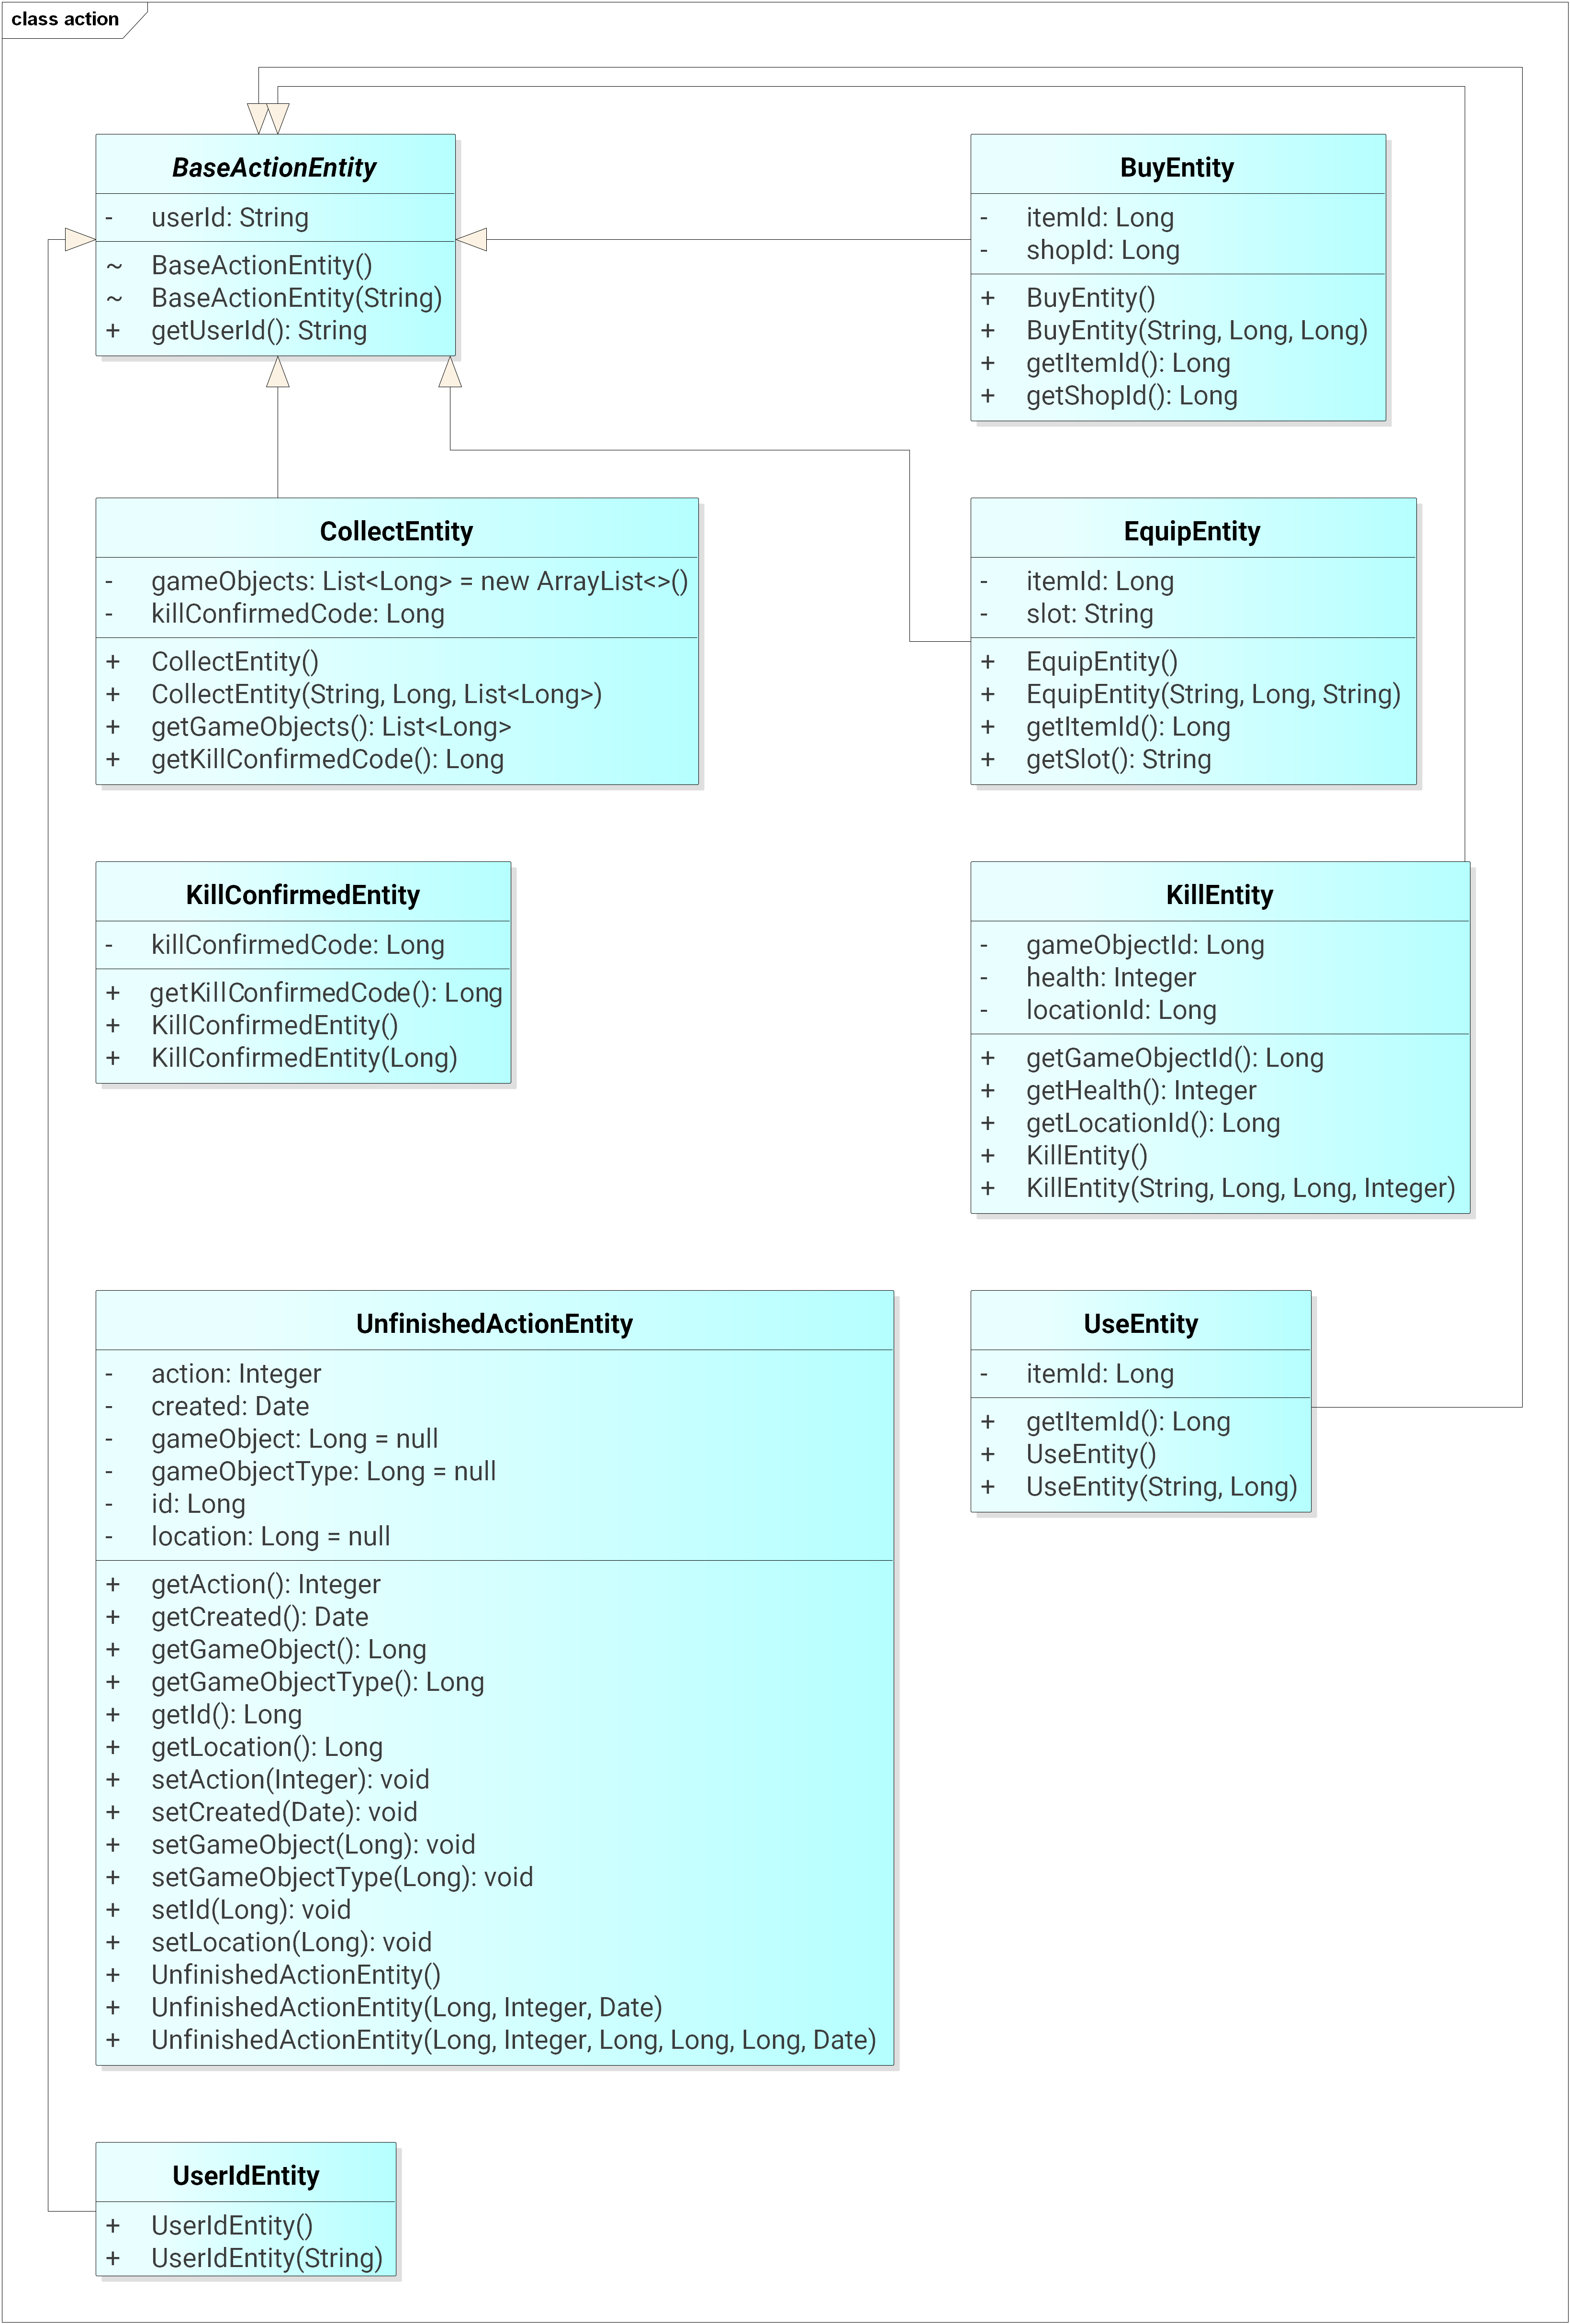
\includegraphics[width=\textwidth]{figures/classdiagrams/dsaction}
	\centering			
	\caption{Class diagram of package \textit{bachelors.database.api.action}}
\end{figure}

\begin{figure}[h]	
	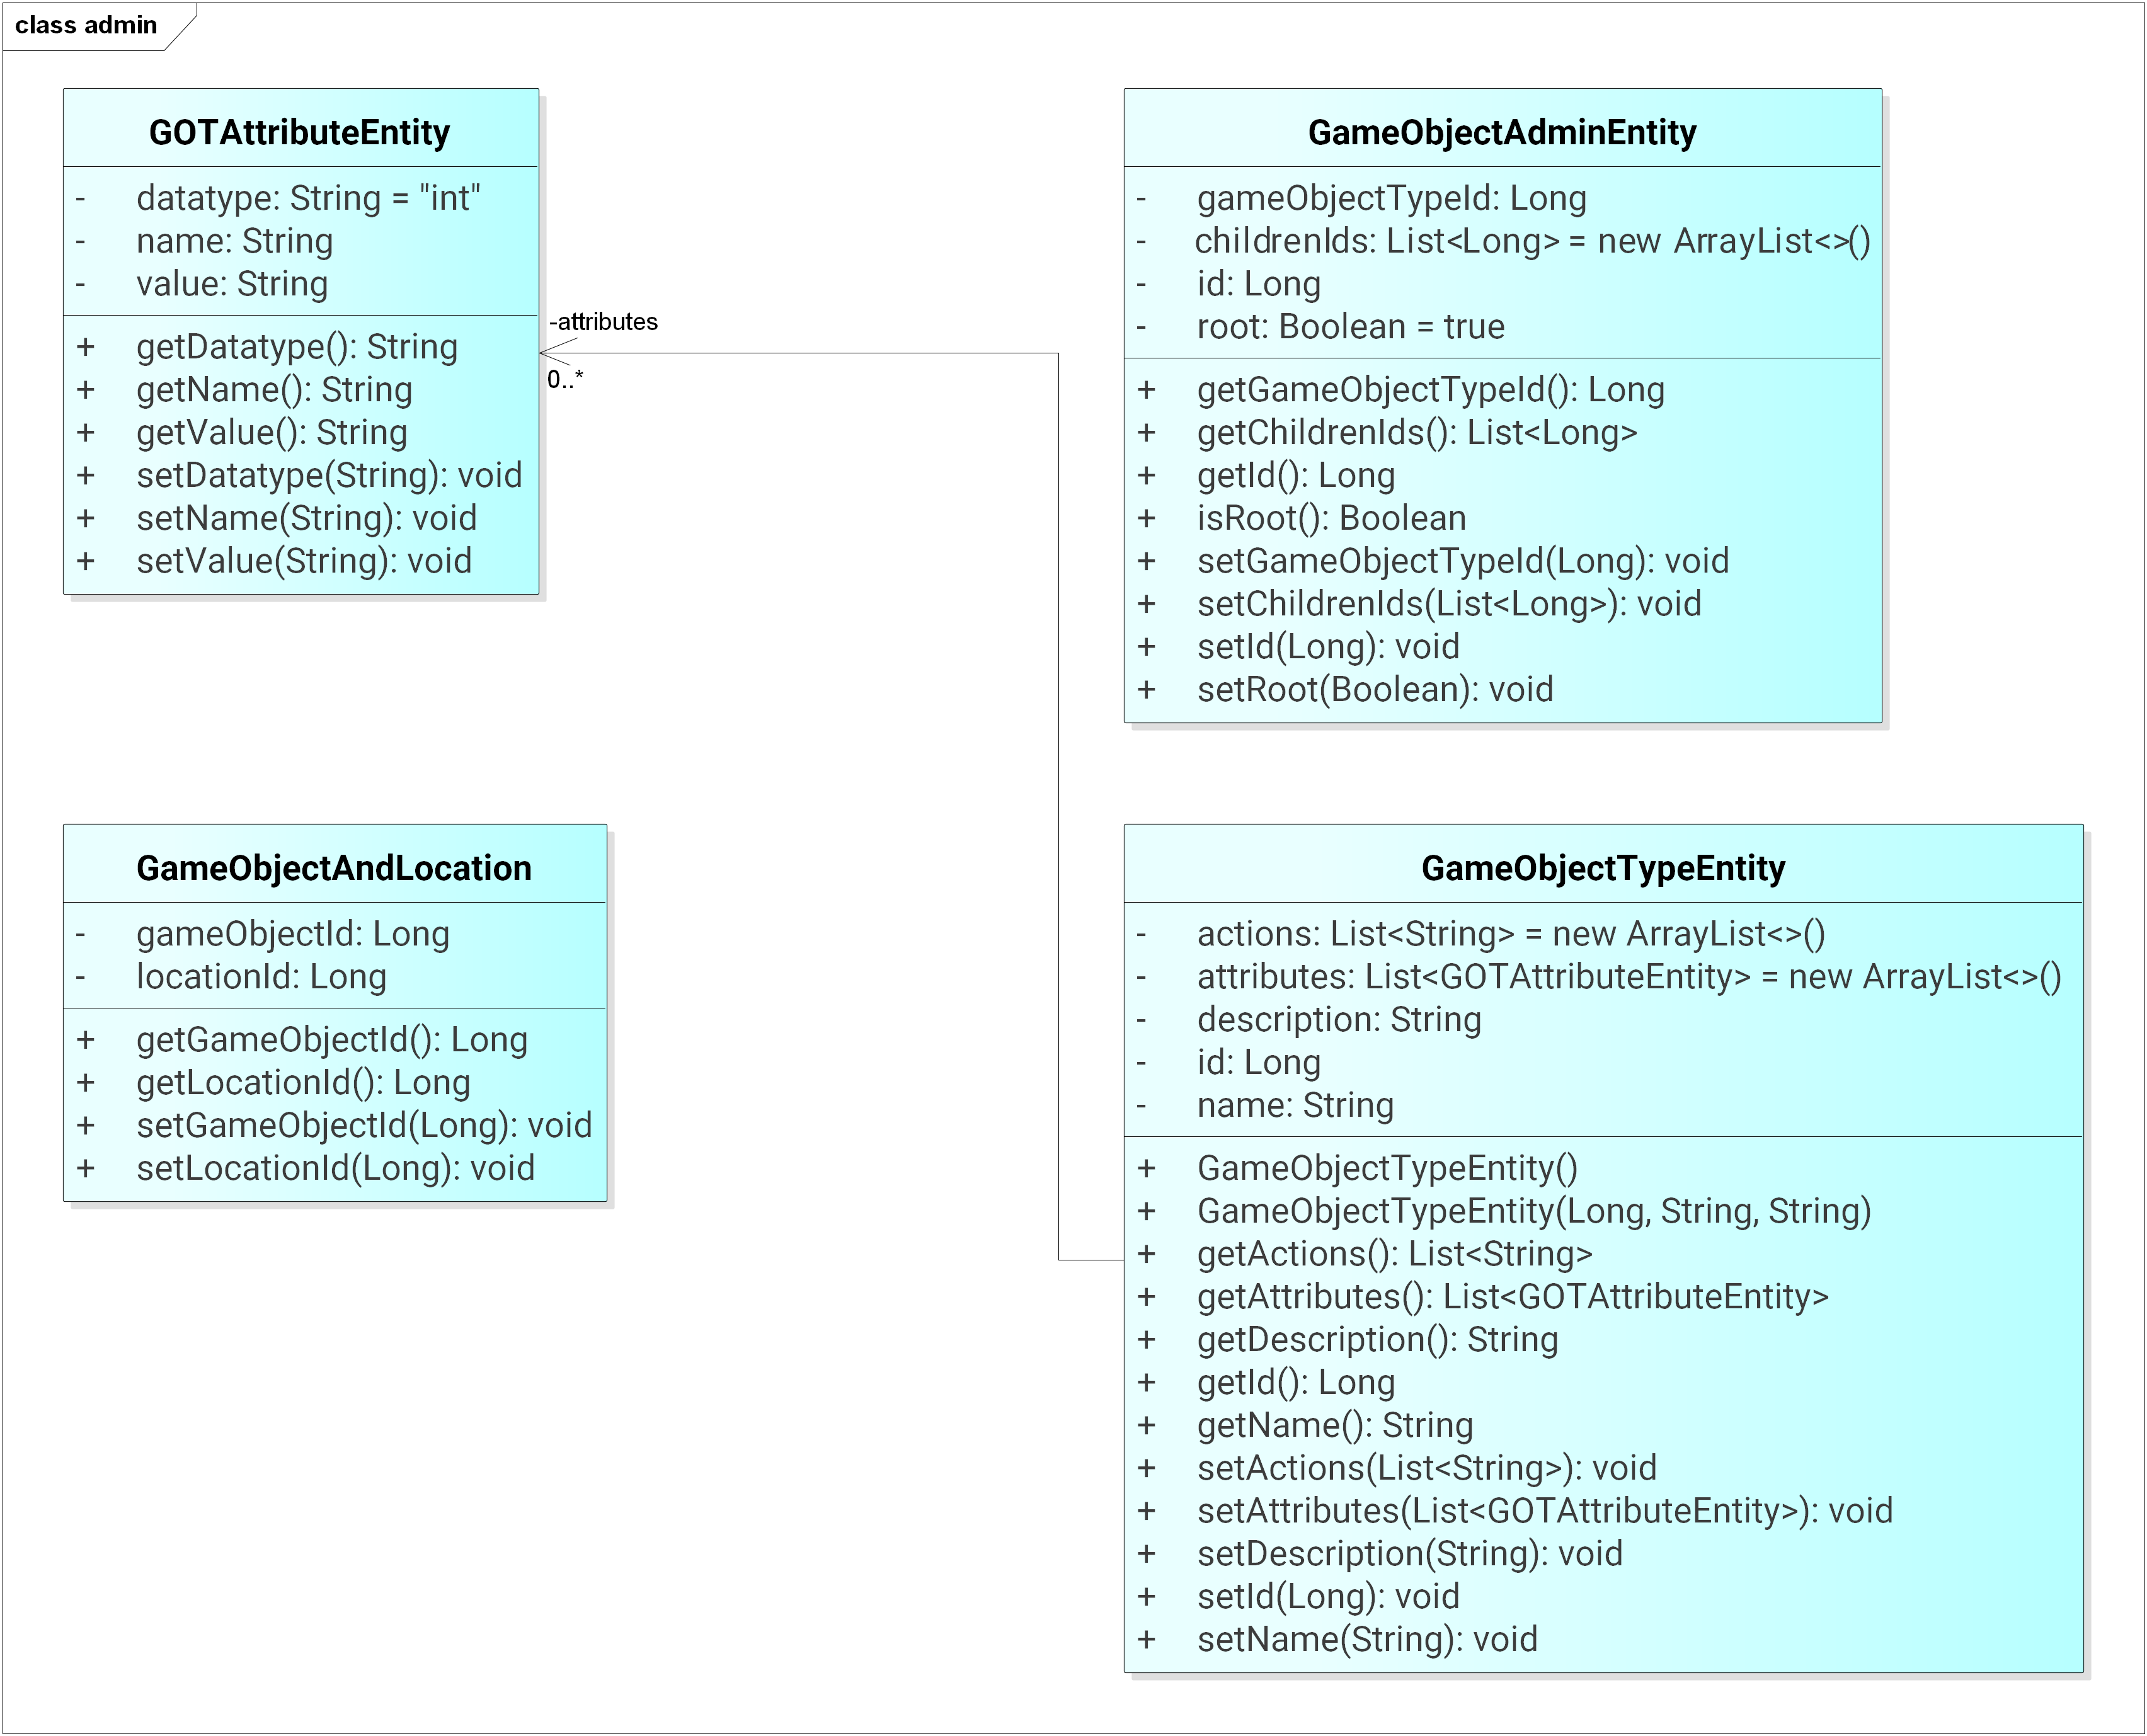
\includegraphics[width=\textwidth]{figures/classdiagrams/dsadmin}
	\centering			
	\caption{Class diagram of package \textit{bachelors.database.admin}}
\end{figure}

\begin{figure}[h]	
	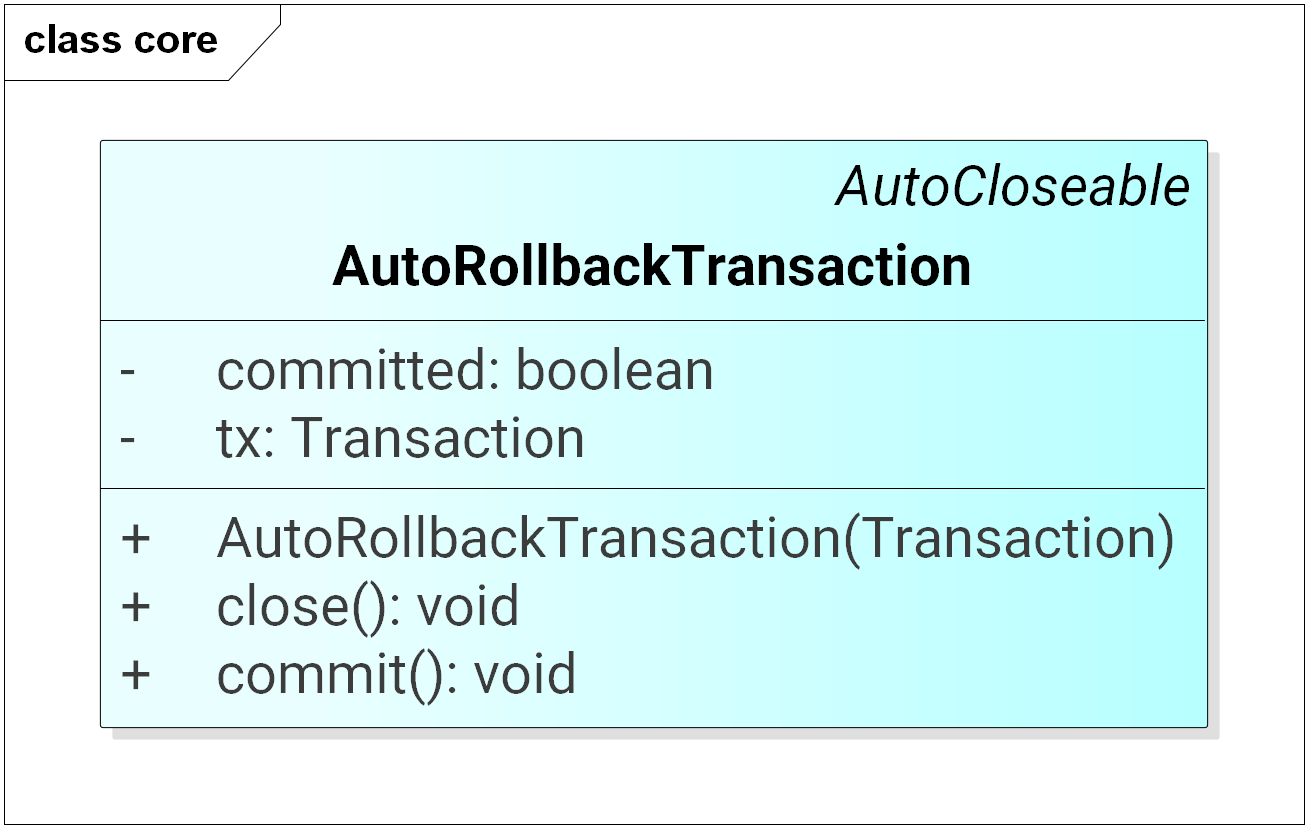
\includegraphics[width=0.6\textwidth]{figures/classdiagrams/dscore}
	\centering			
	\caption{Class diagram of package \textit{bachelors.database.core}}
\end{figure}

\begin{figure}[h]	
	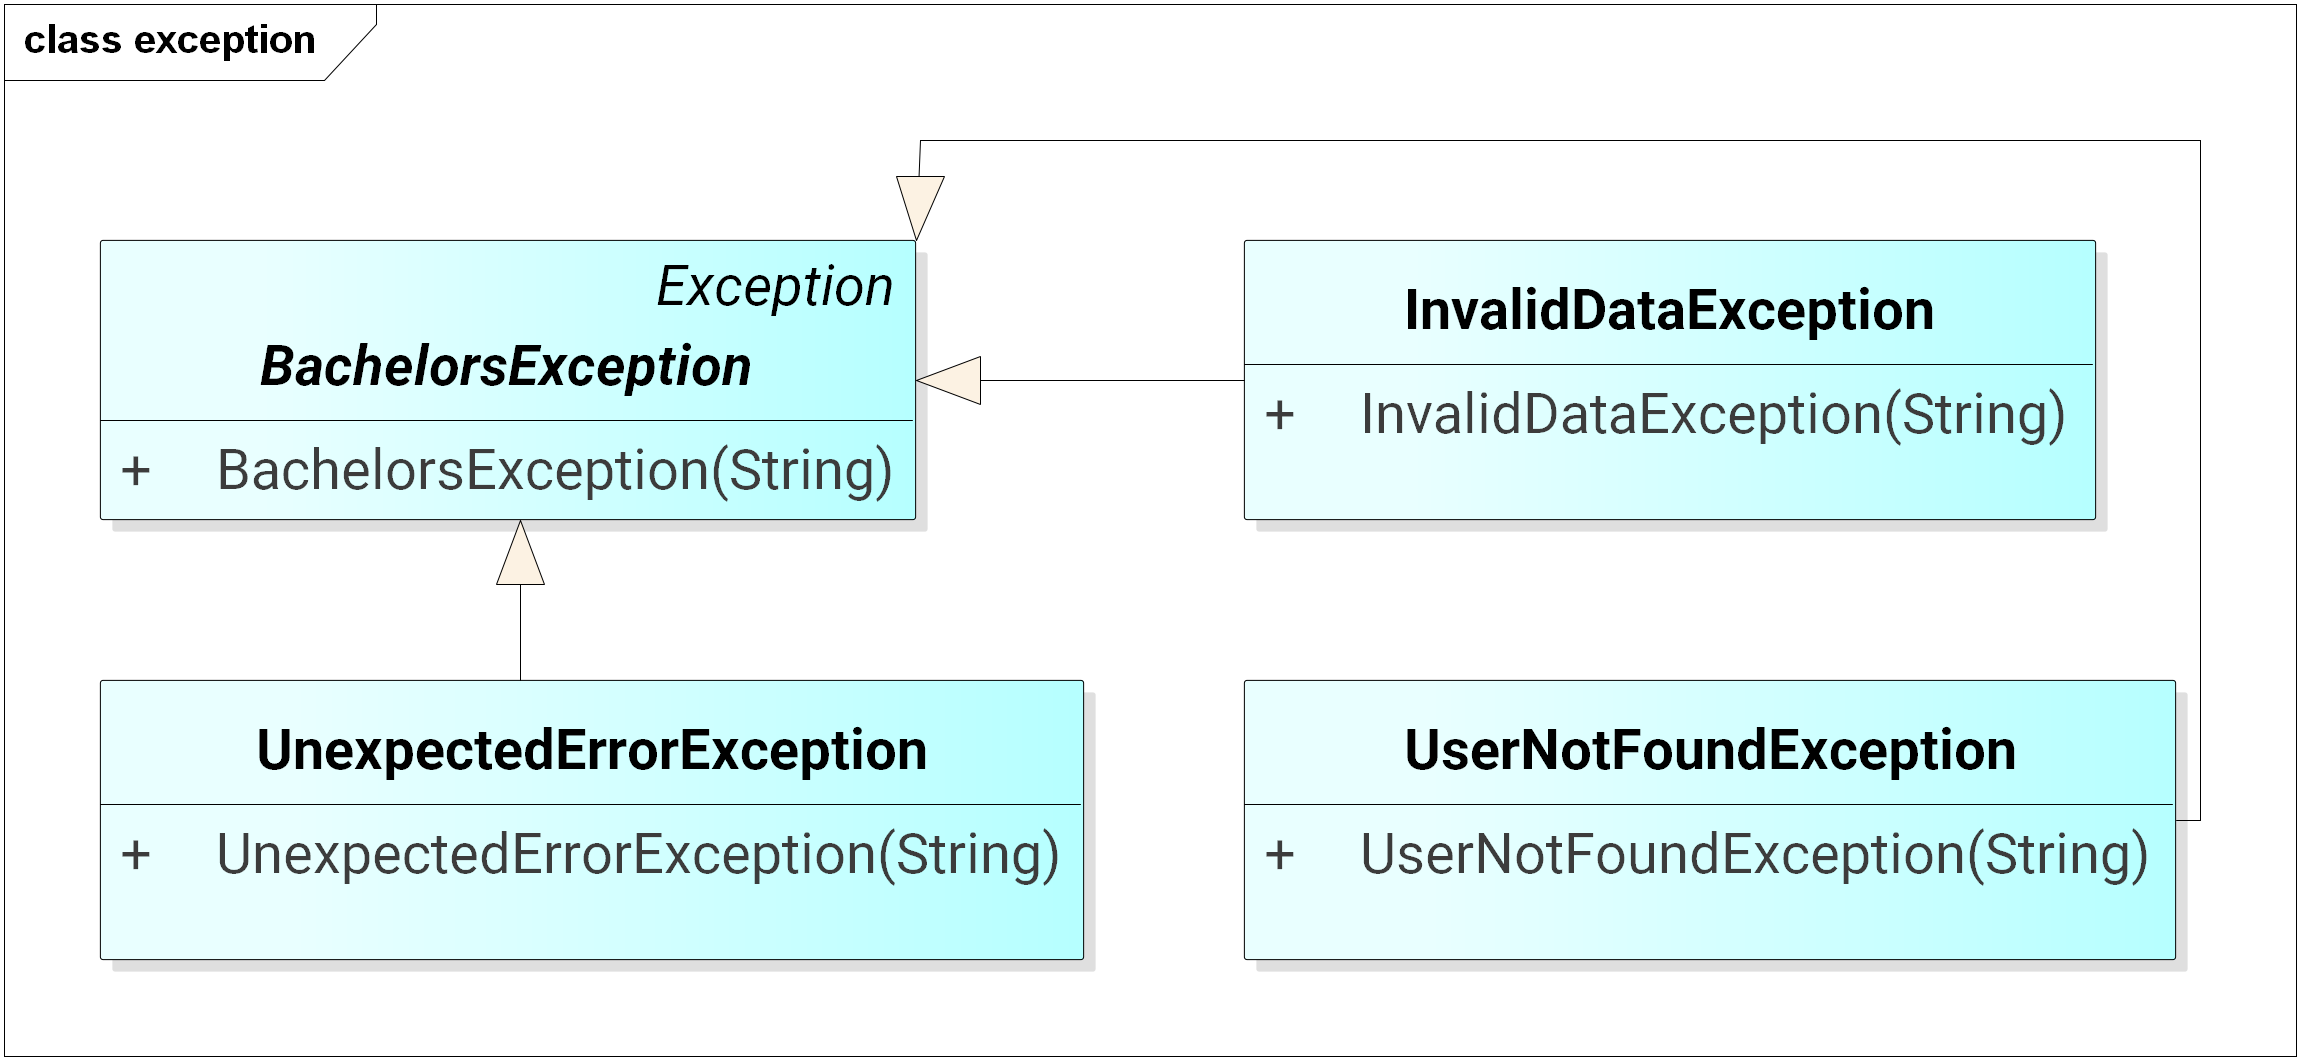
\includegraphics[width=\textwidth]{figures/classdiagrams/dsexception}
	\centering			
	\caption{Class diagram of package \textit{bachelors.database.exception}}
\end{figure}

\begin{figure}[h]	
	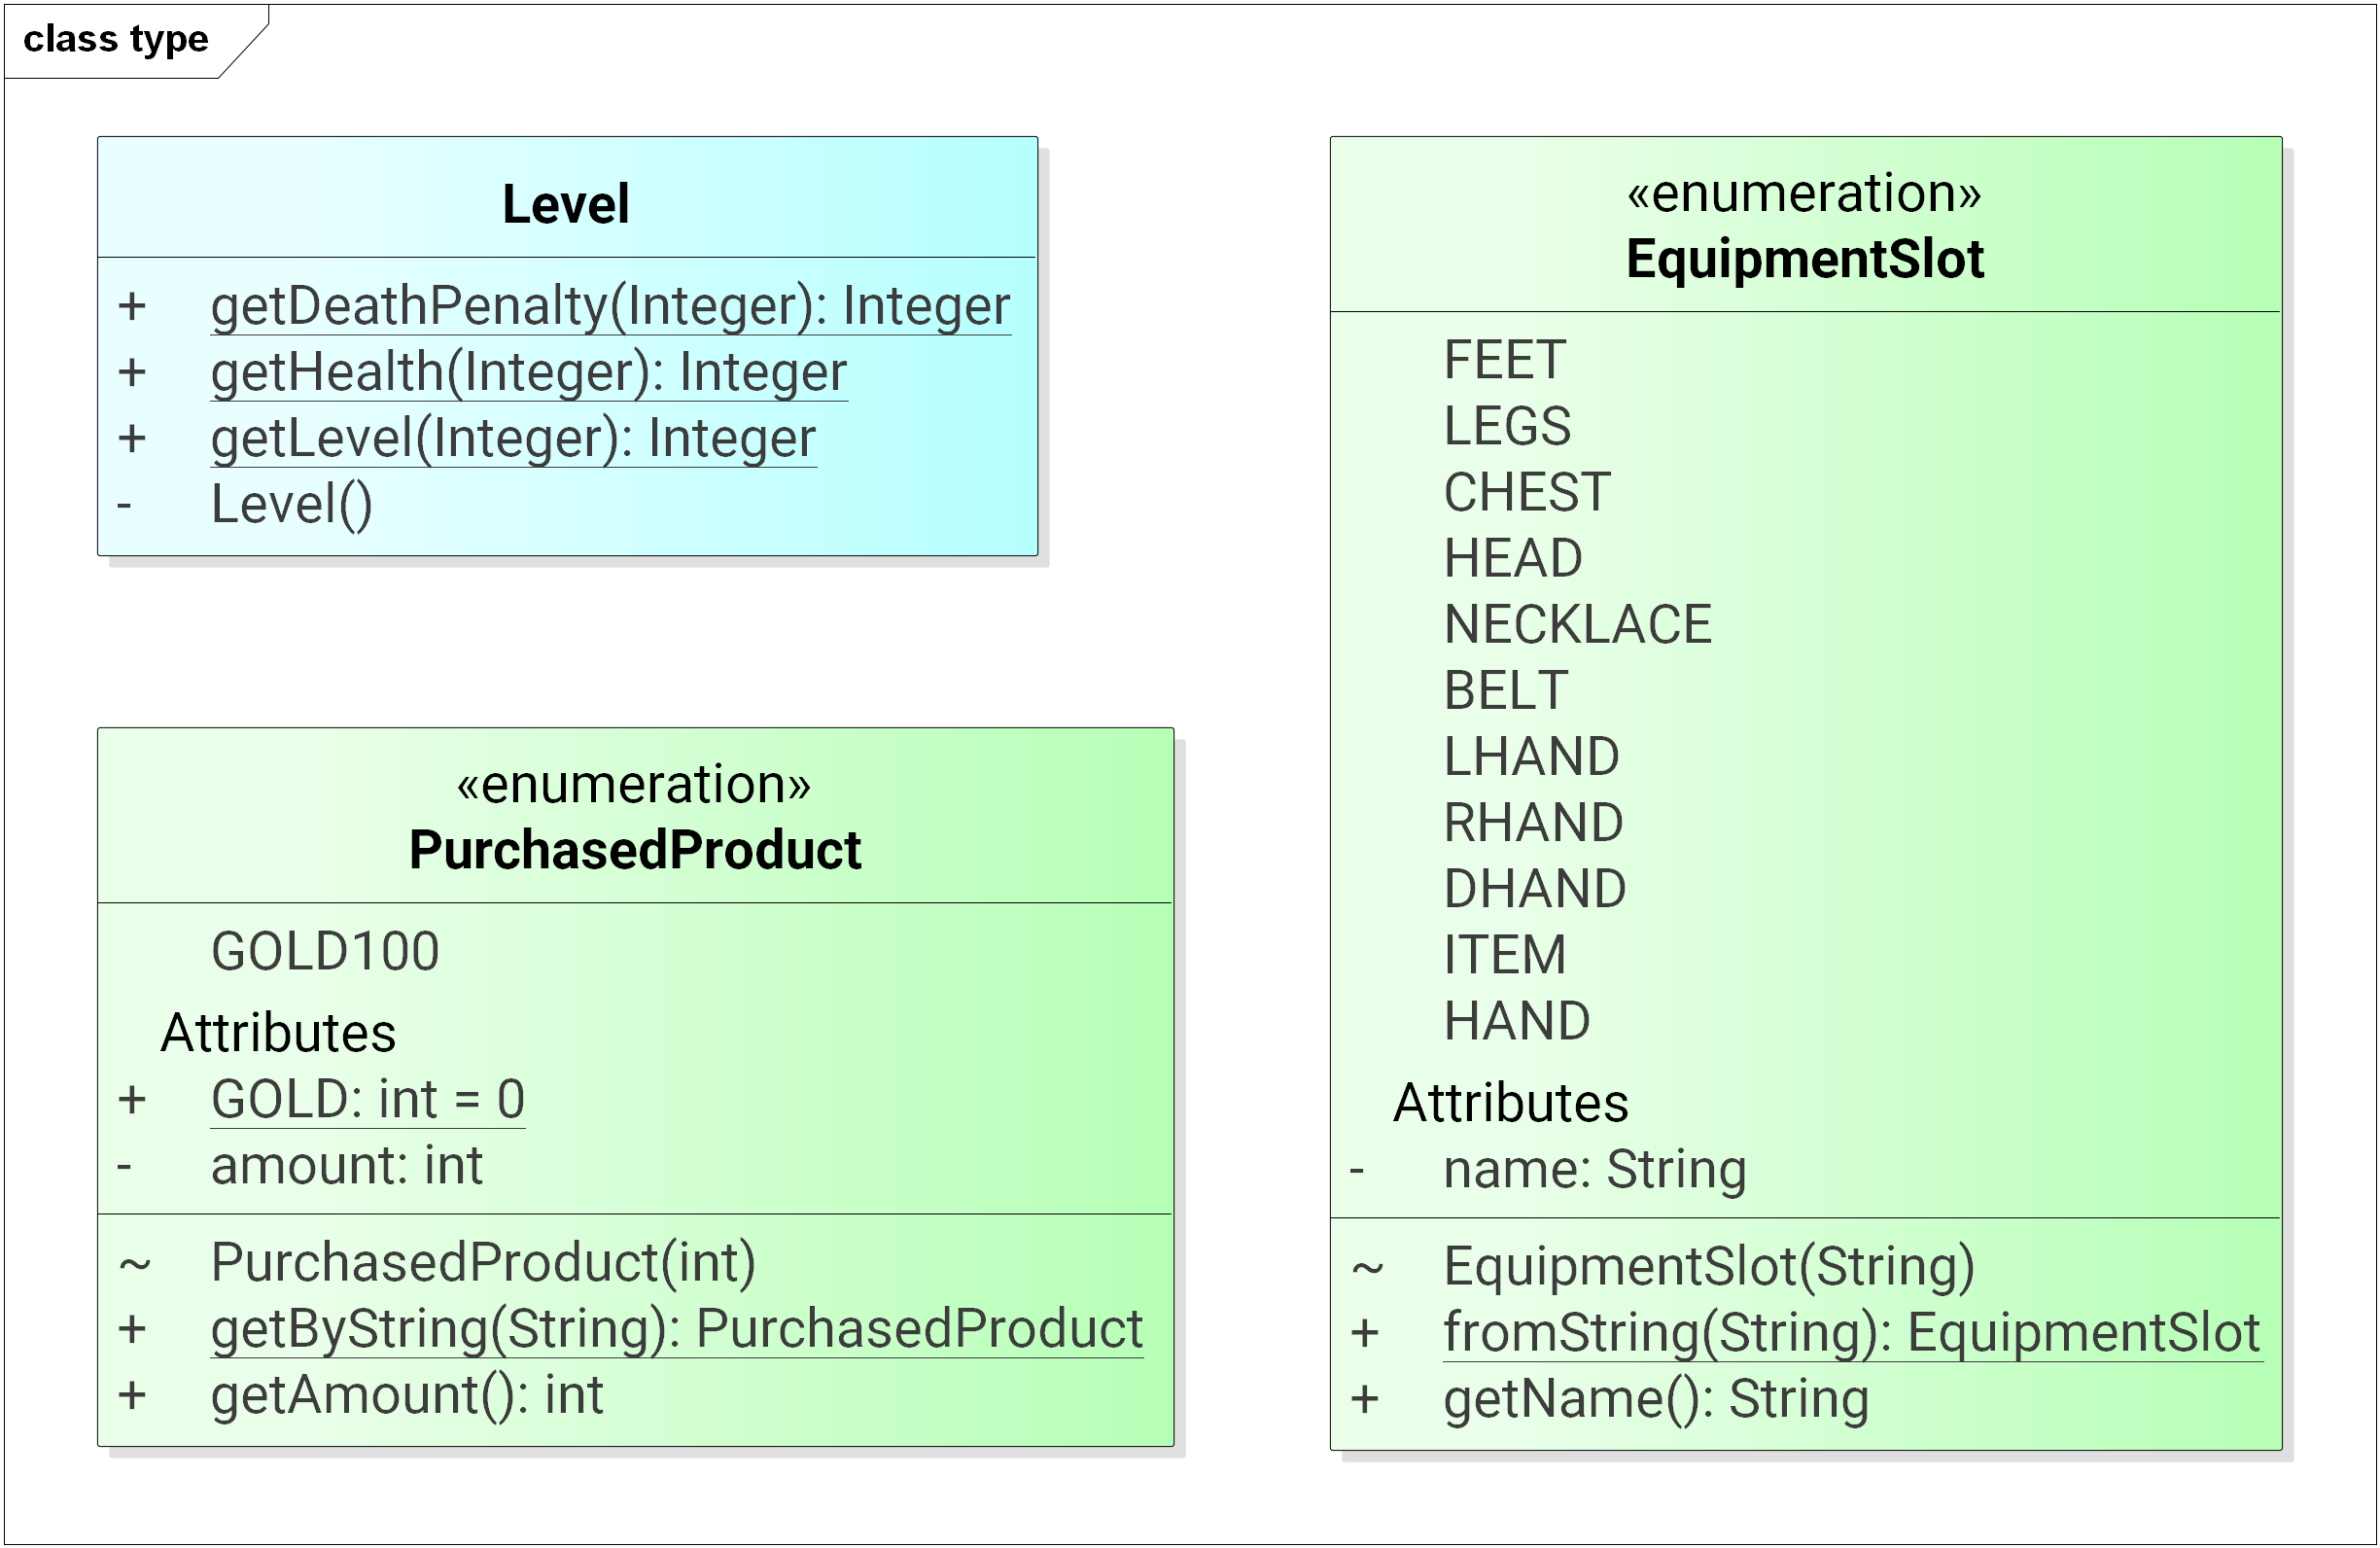
\includegraphics[width=\textwidth]{figures/classdiagrams/dstype}
	\centering			
	\caption{Class diagram of package \textit{bachelors.database.type}}
\end{figure}

\begin{figure}[h]	
	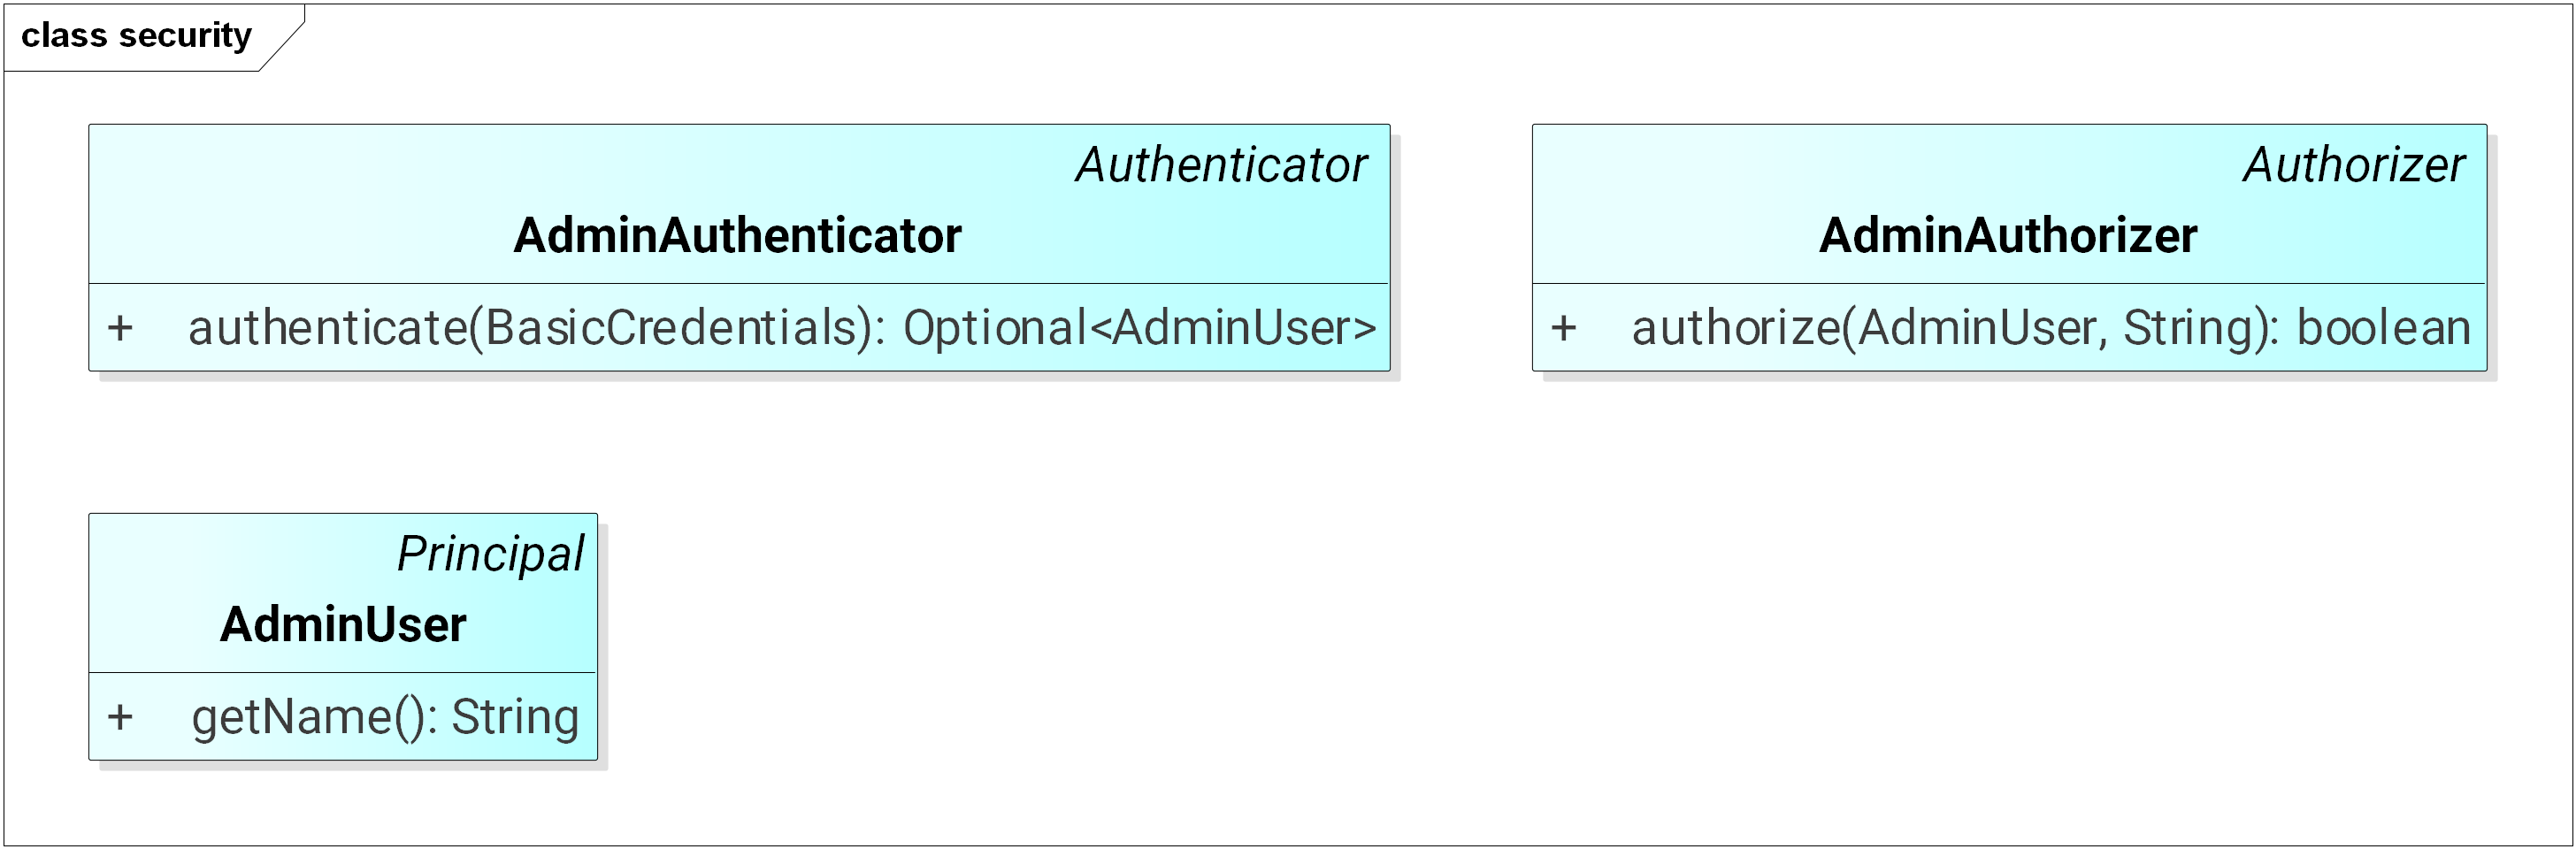
\includegraphics[width=\textwidth]{figures/classdiagrams/dssecurity}
	\centering			
	\caption{Class diagram of package \textit{bachelors.database.security}}
\end{figure}

\begin{figure}[h]	
	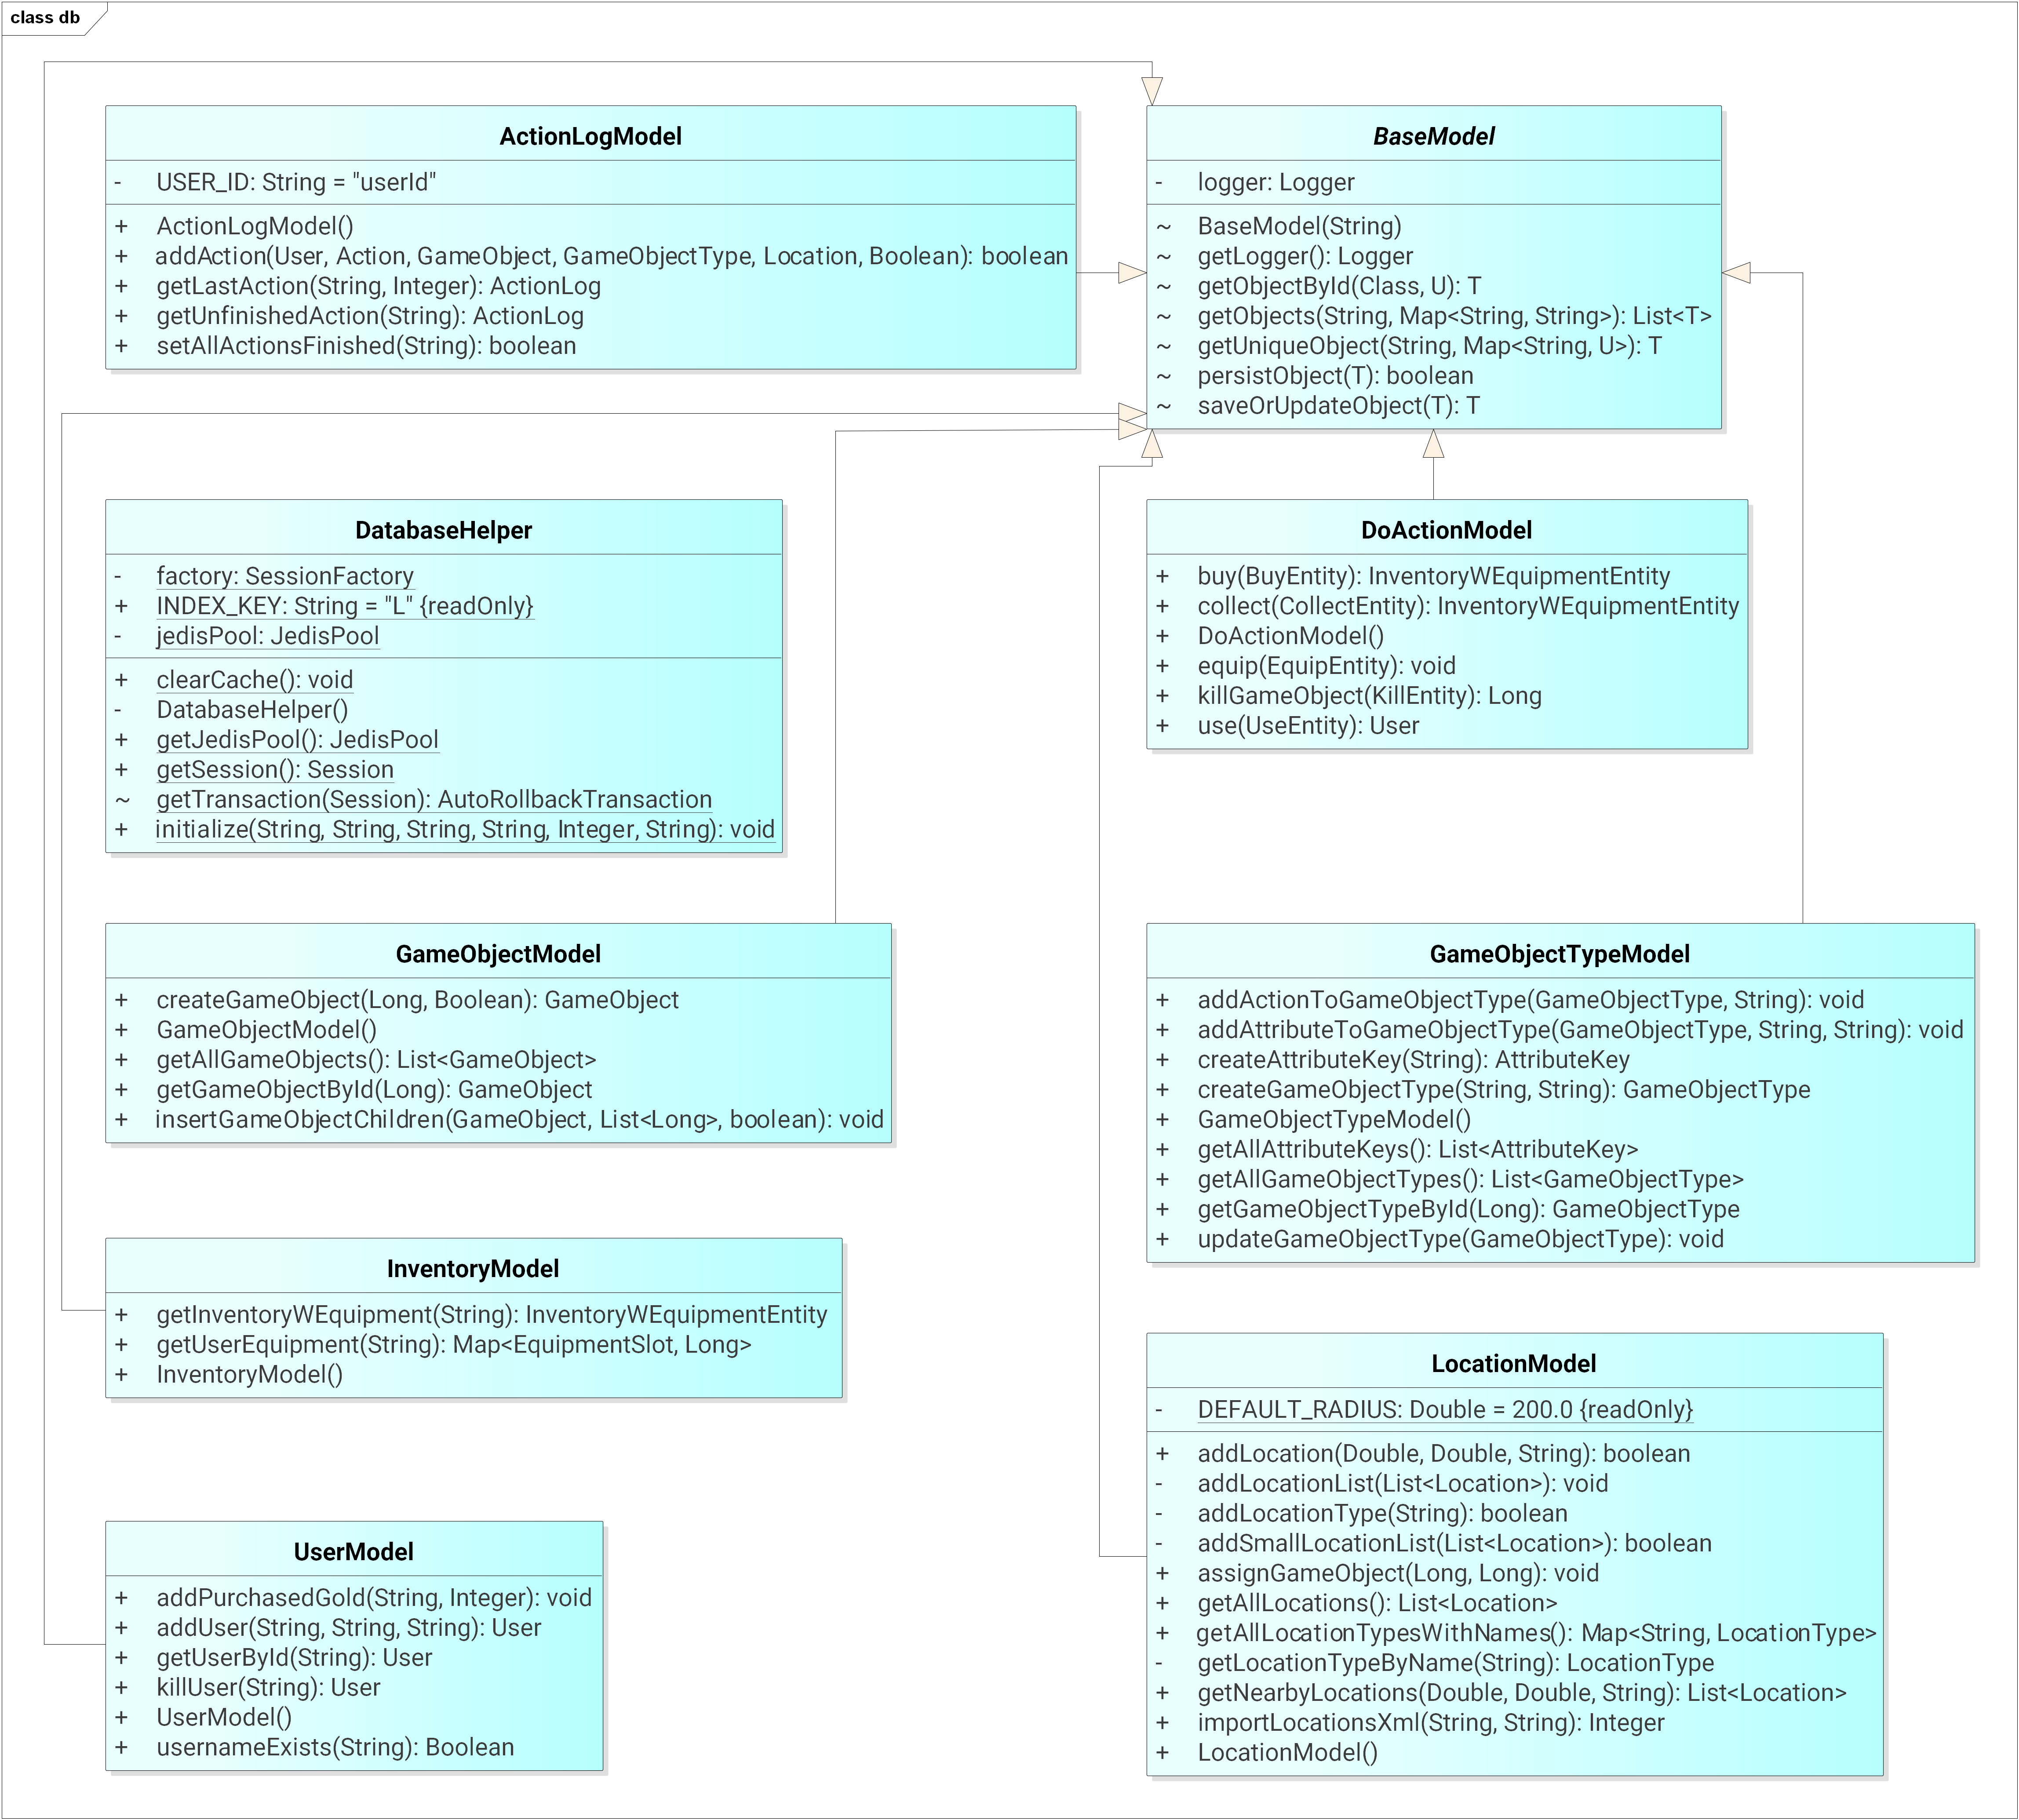
\includegraphics[width=\textwidth]{figures/classdiagrams/dsdb}
	\centering			
	\caption{Class diagram of package \textit{bachelors.database.db}}
\end{figure}

\begin{figure}[h]	
	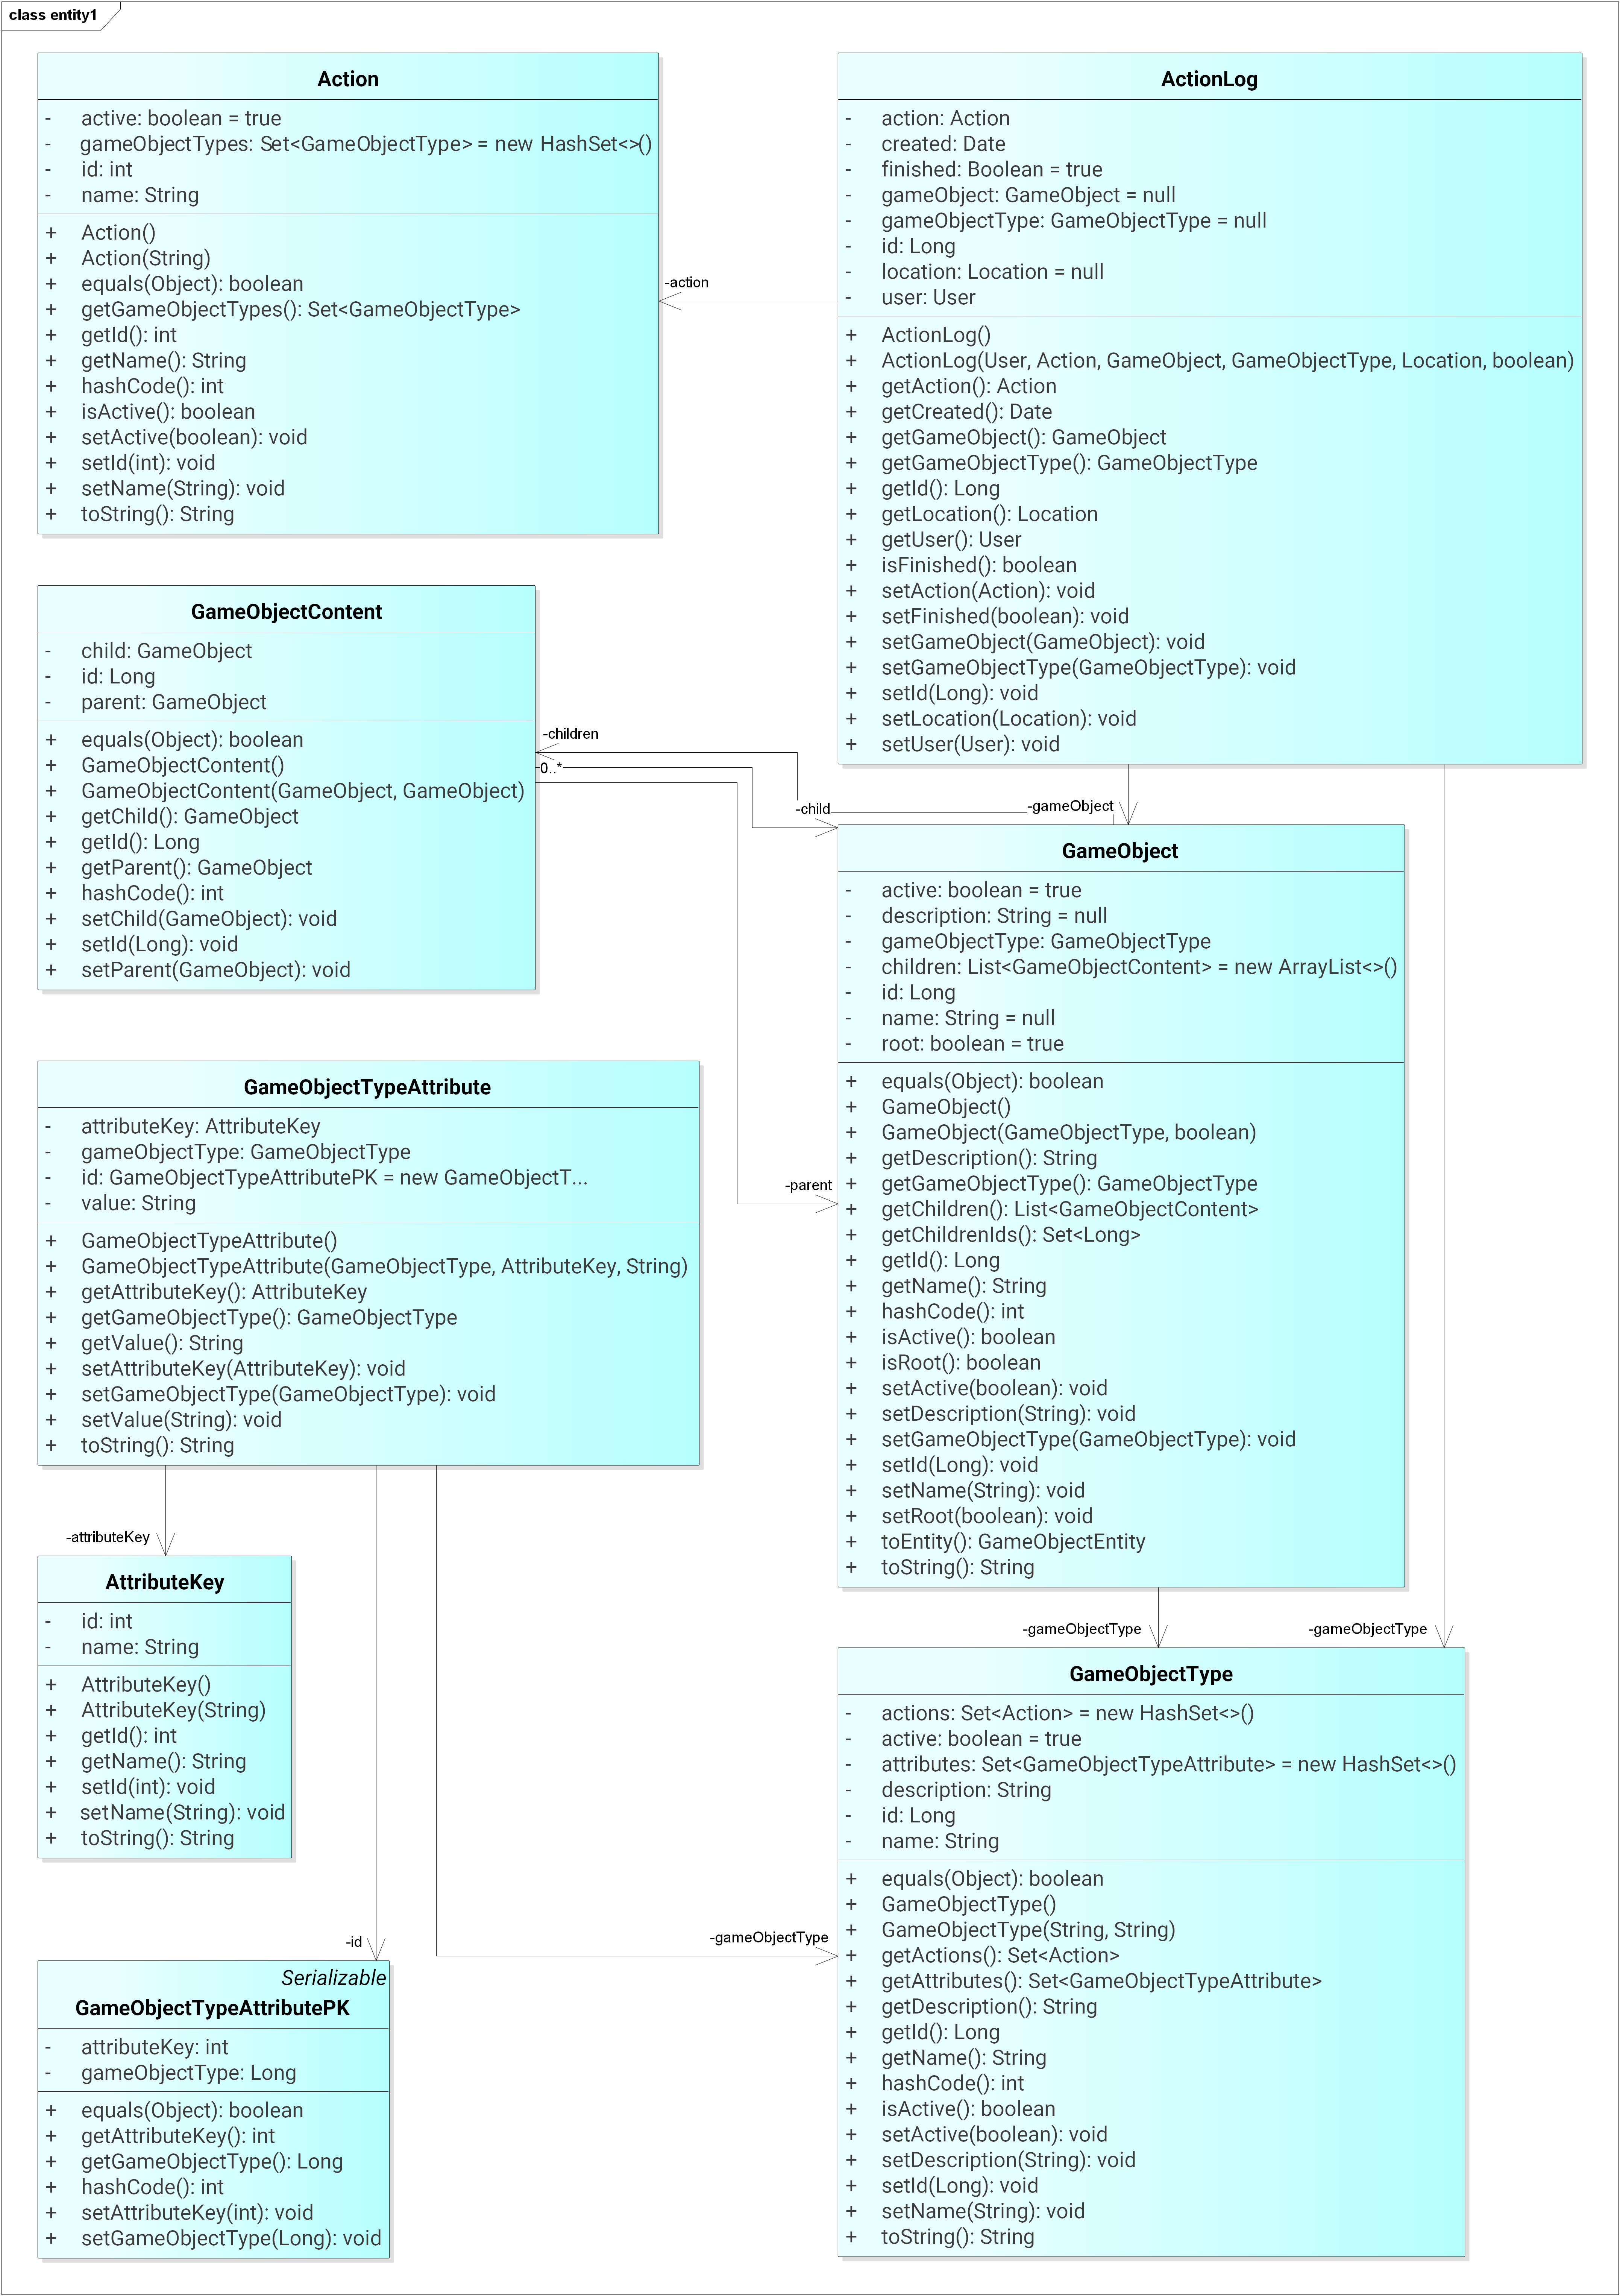
\includegraphics[width=\textwidth]{figures/classdiagrams/dsentity1}
	\centering			
	\caption{Part 1/3 of a class diagram of package \textit{bachelors.database.entity}}
\end{figure}

\begin{figure}[h]	
	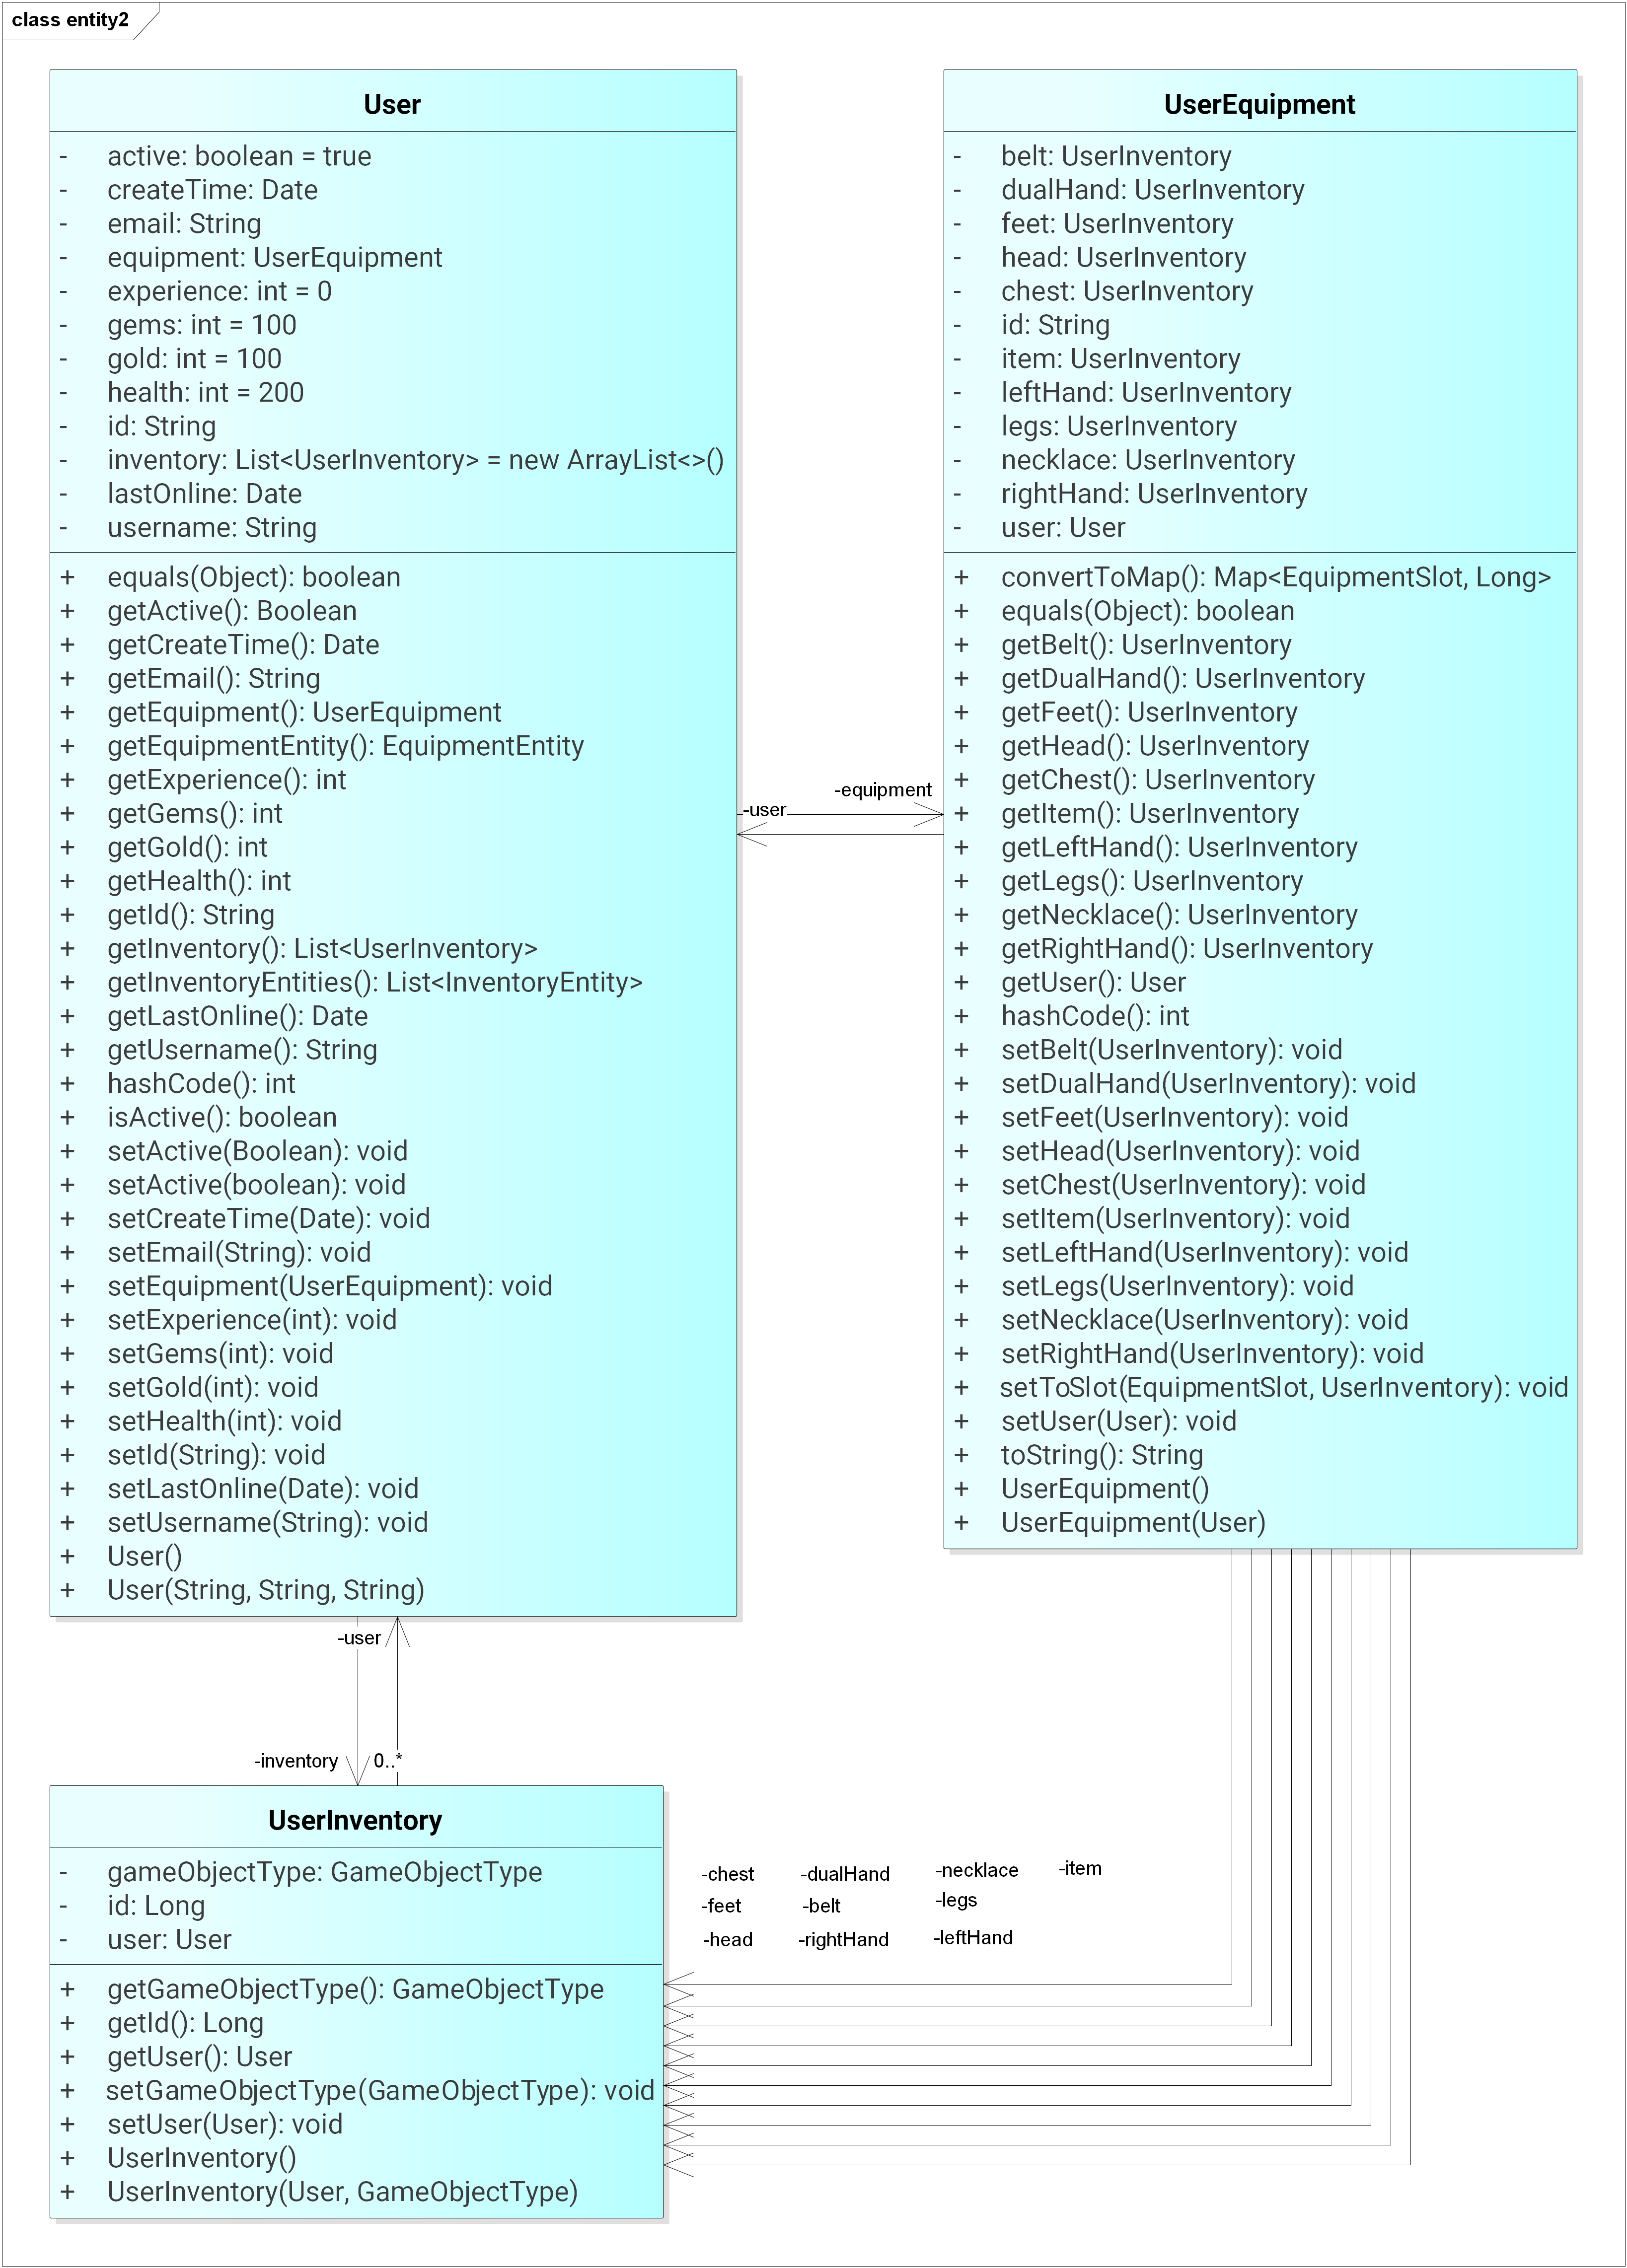
\includegraphics[width=\textwidth]{figures/classdiagrams/dsentity2}
	\centering			
	\caption{Part 2/3 of a class diagram of package \textit{bachelors.database.entity}}
\end{figure}

\begin{figure}[h]	
	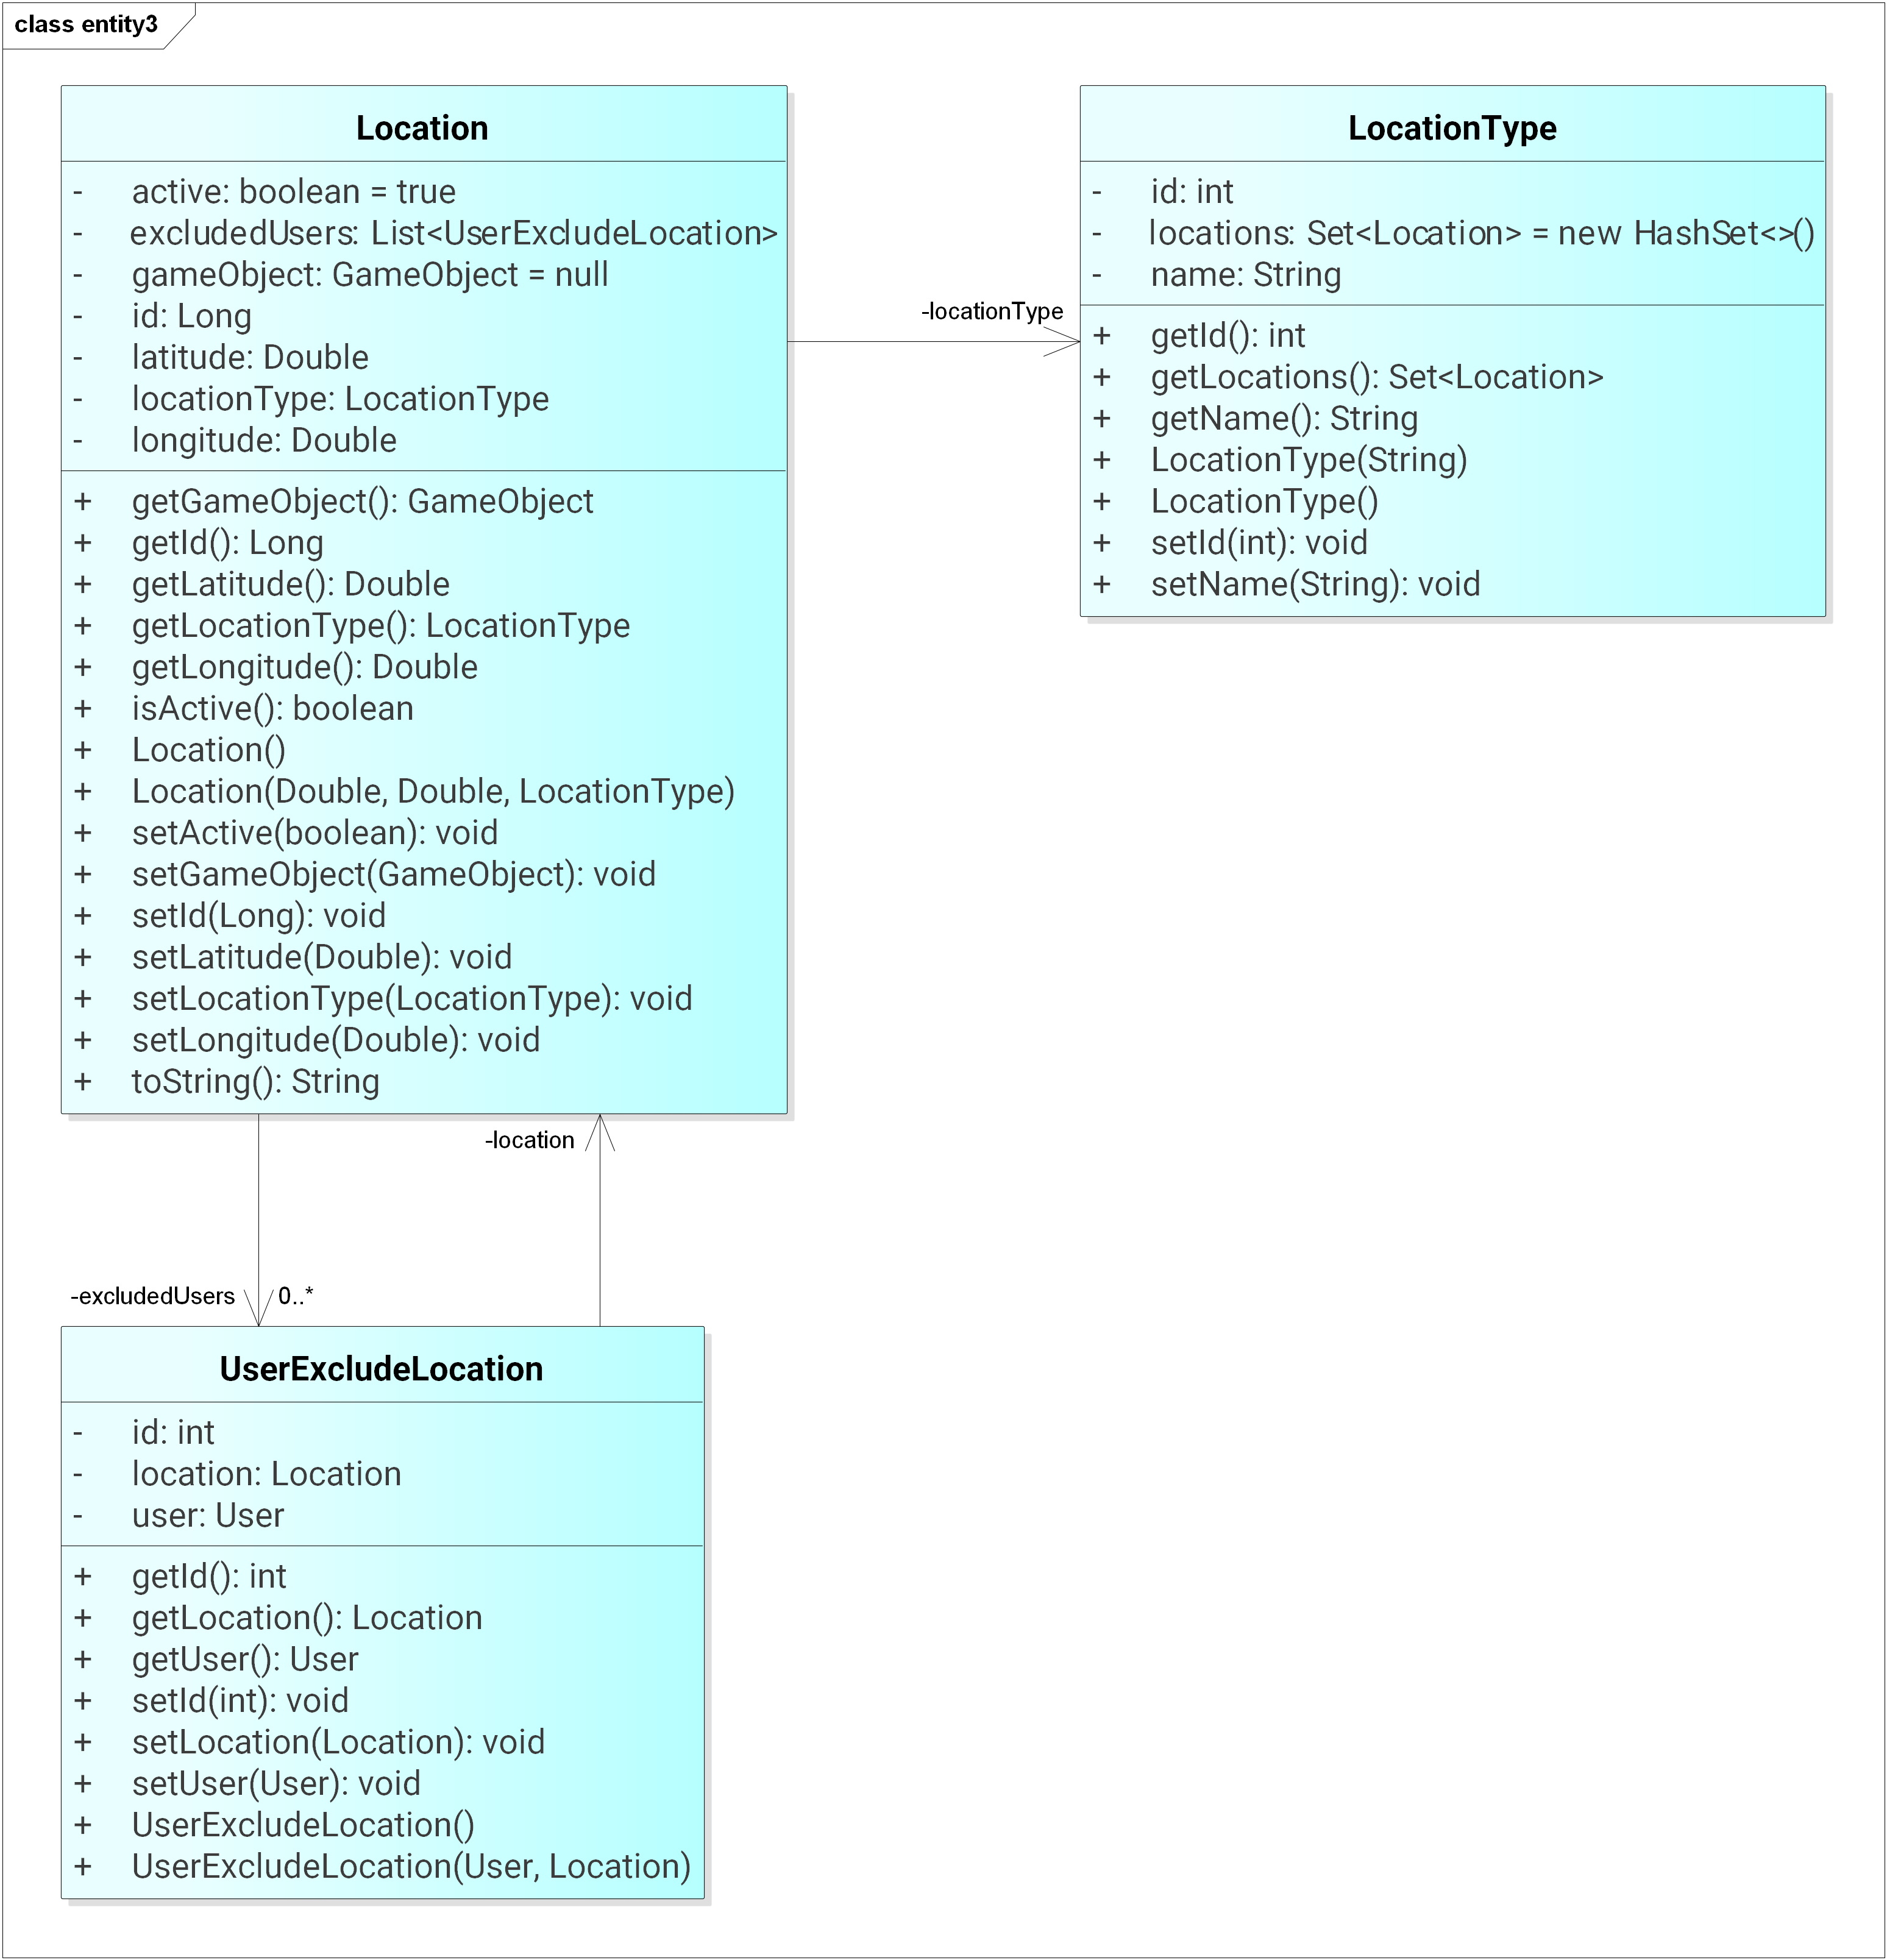
\includegraphics[width=\textwidth]{figures/classdiagrams/dsentity3}
	\centering			
	\caption{Part 3/3 of a class diagram of package \textit{bachelors.database.entity}}
\end{figure}




\section{Login Server}

\begin{figure}[h]	
	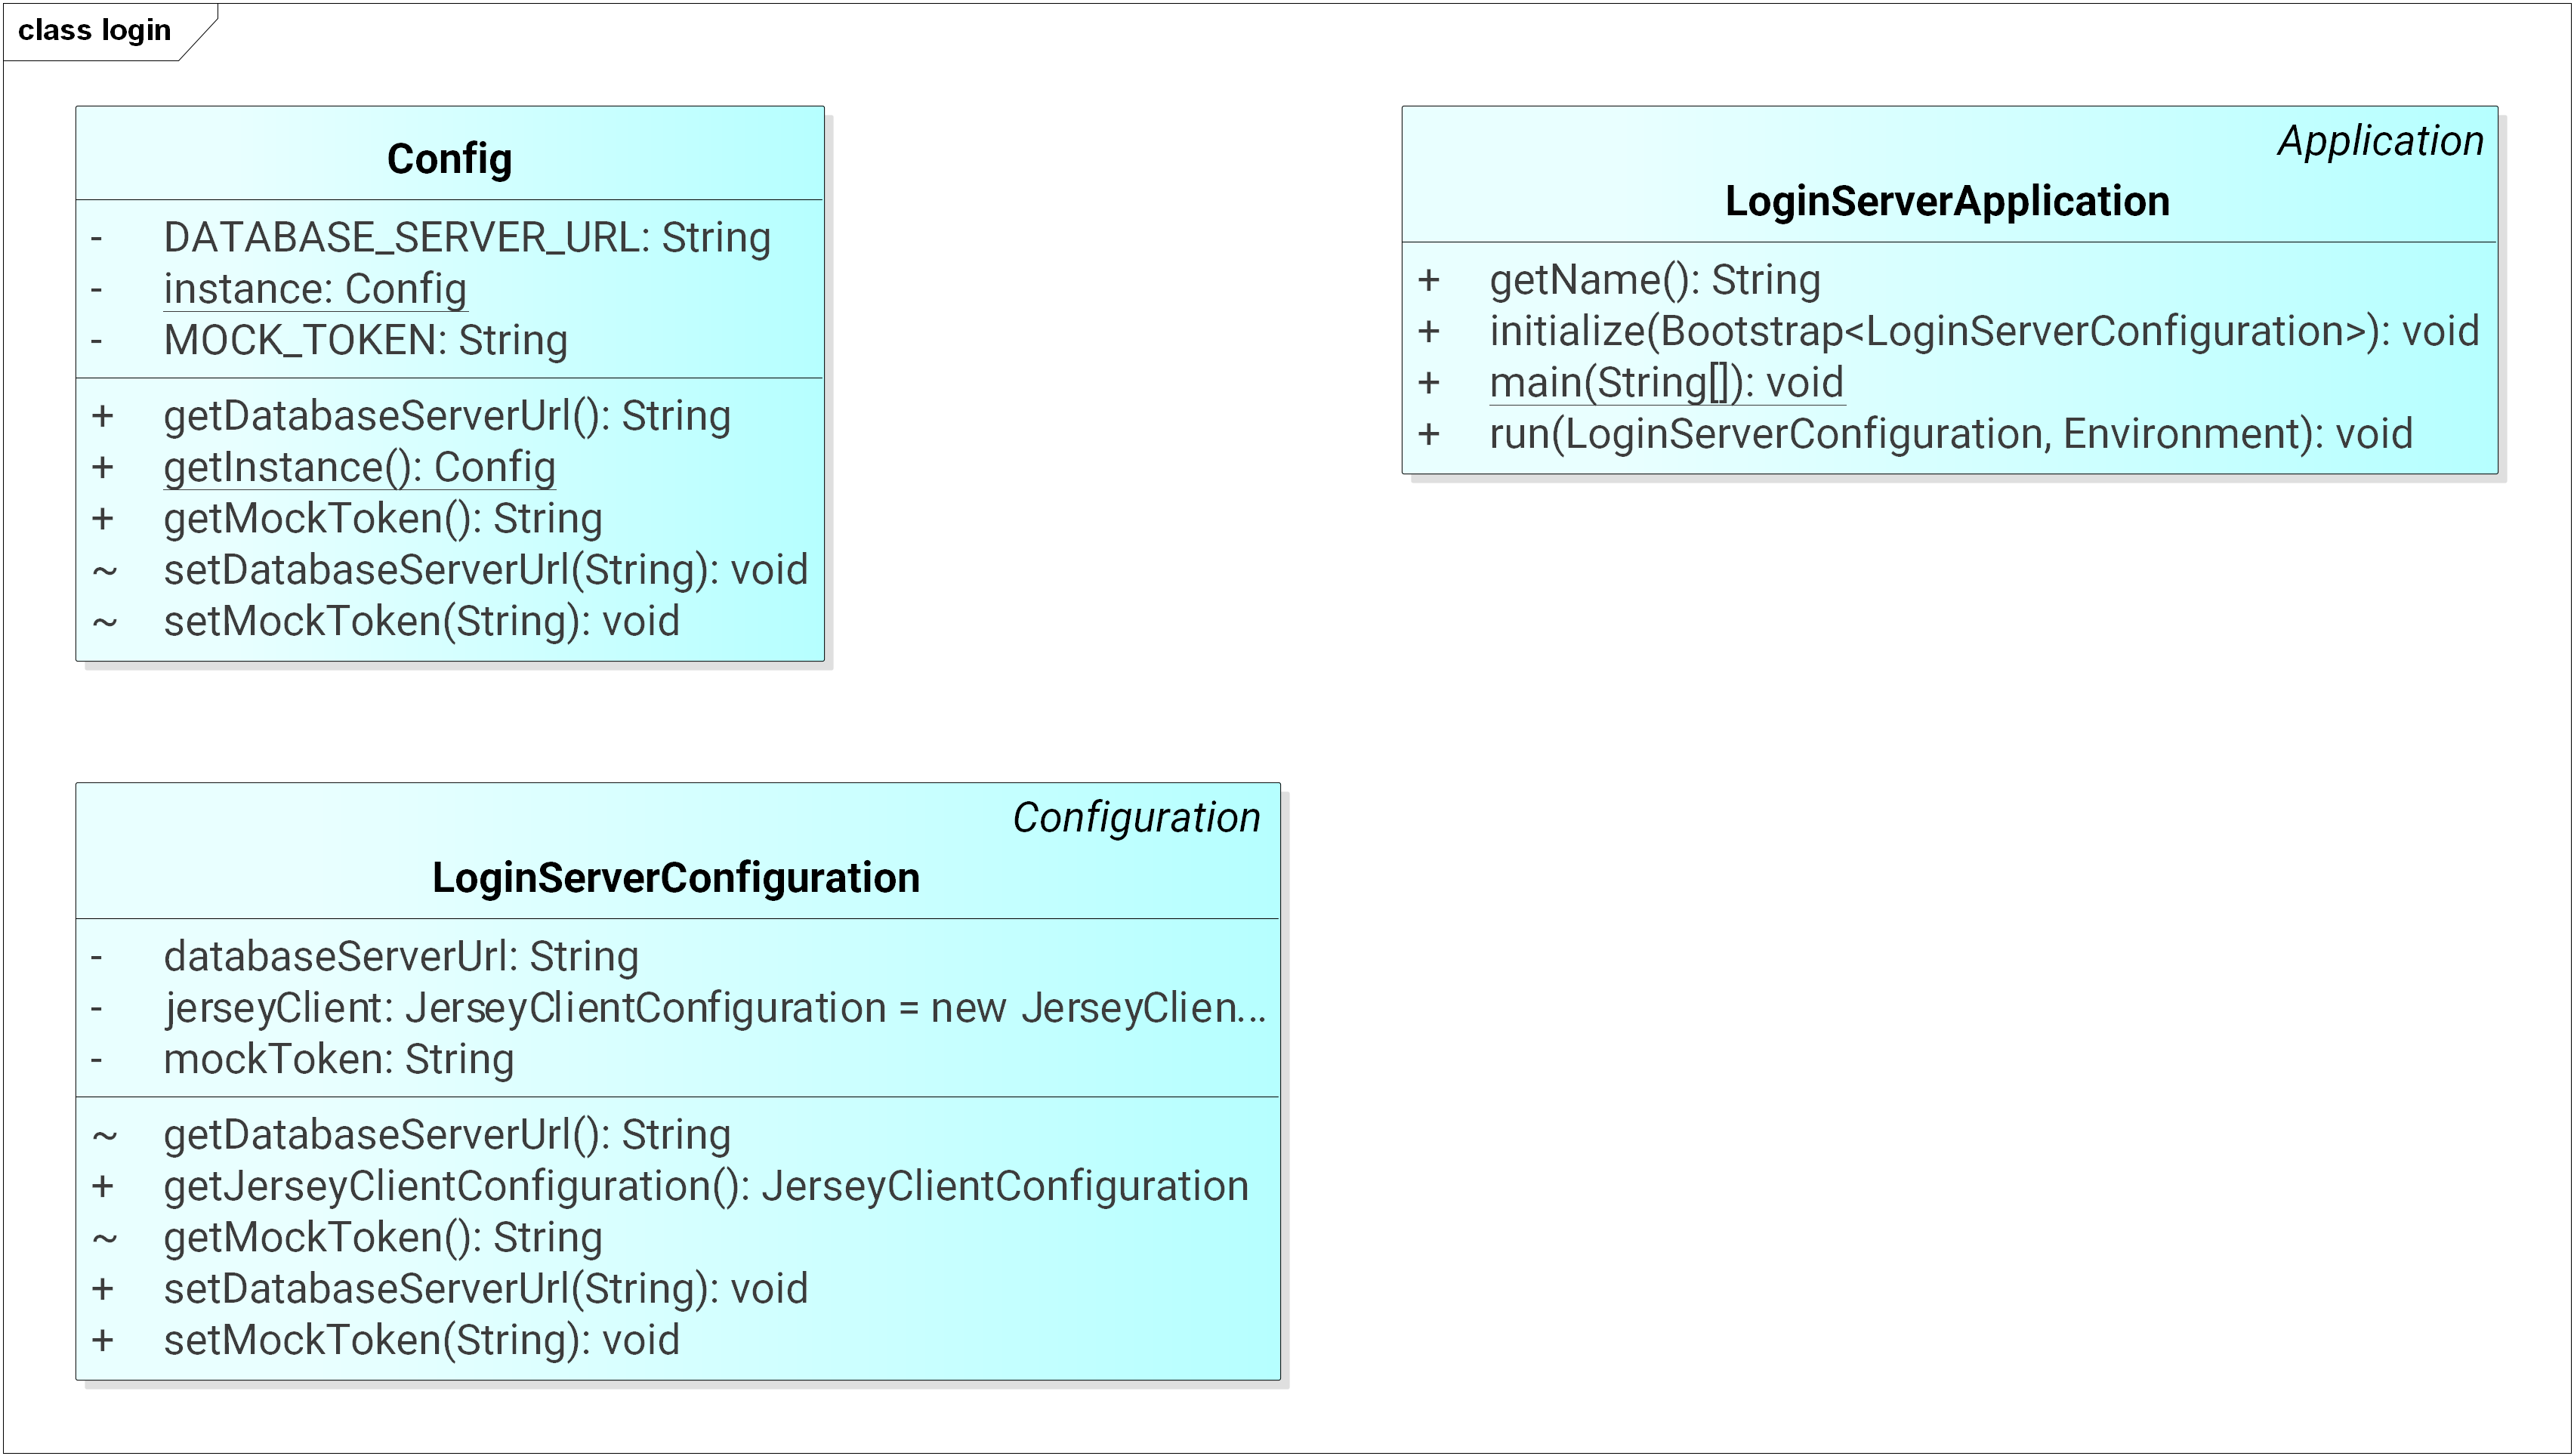
\includegraphics[width=\textwidth]{figures/classdiagrams/lslogin}
	\centering			
	\caption{Class diagram of package \textit{bachelors.login}}
\end{figure}

\begin{figure}[h]	
	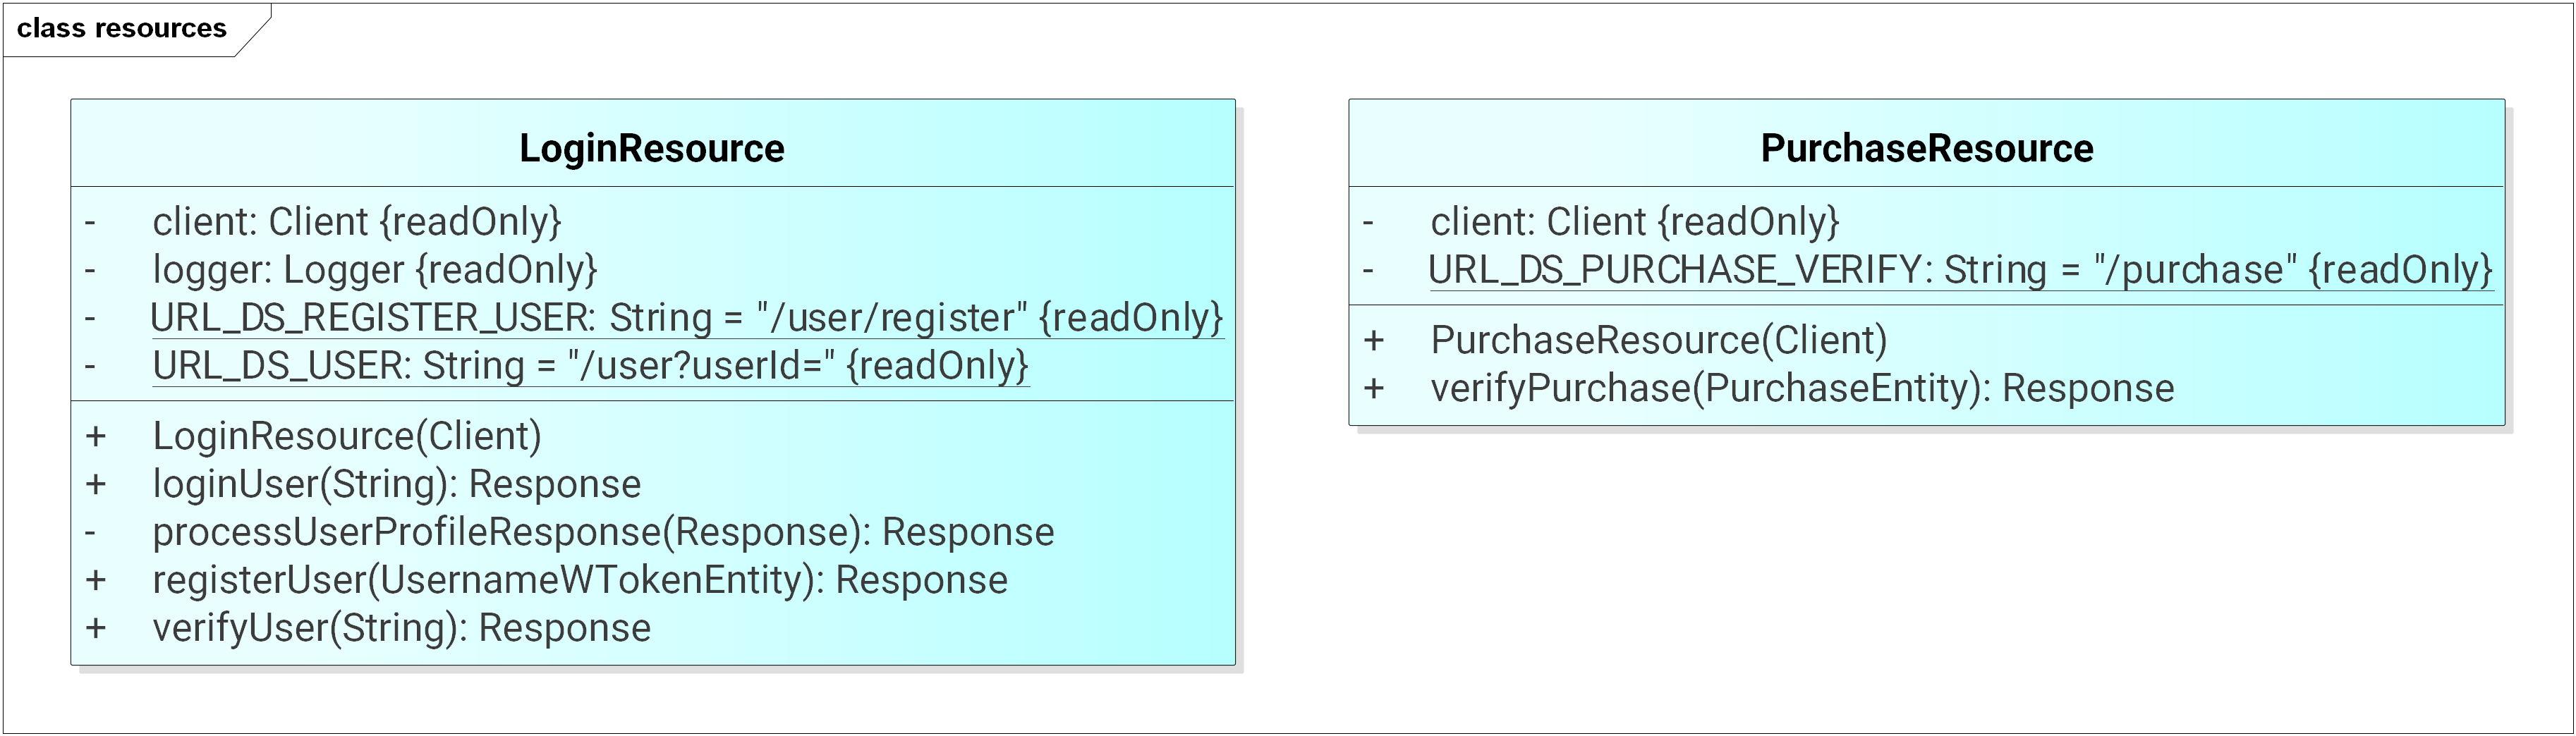
\includegraphics[width=\textwidth]{figures/classdiagrams/lsresources}
	\centering			
	\caption{Class diagram of package \textit{bachelors.login.resources}}
\end{figure}

\begin{figure}[h]	
	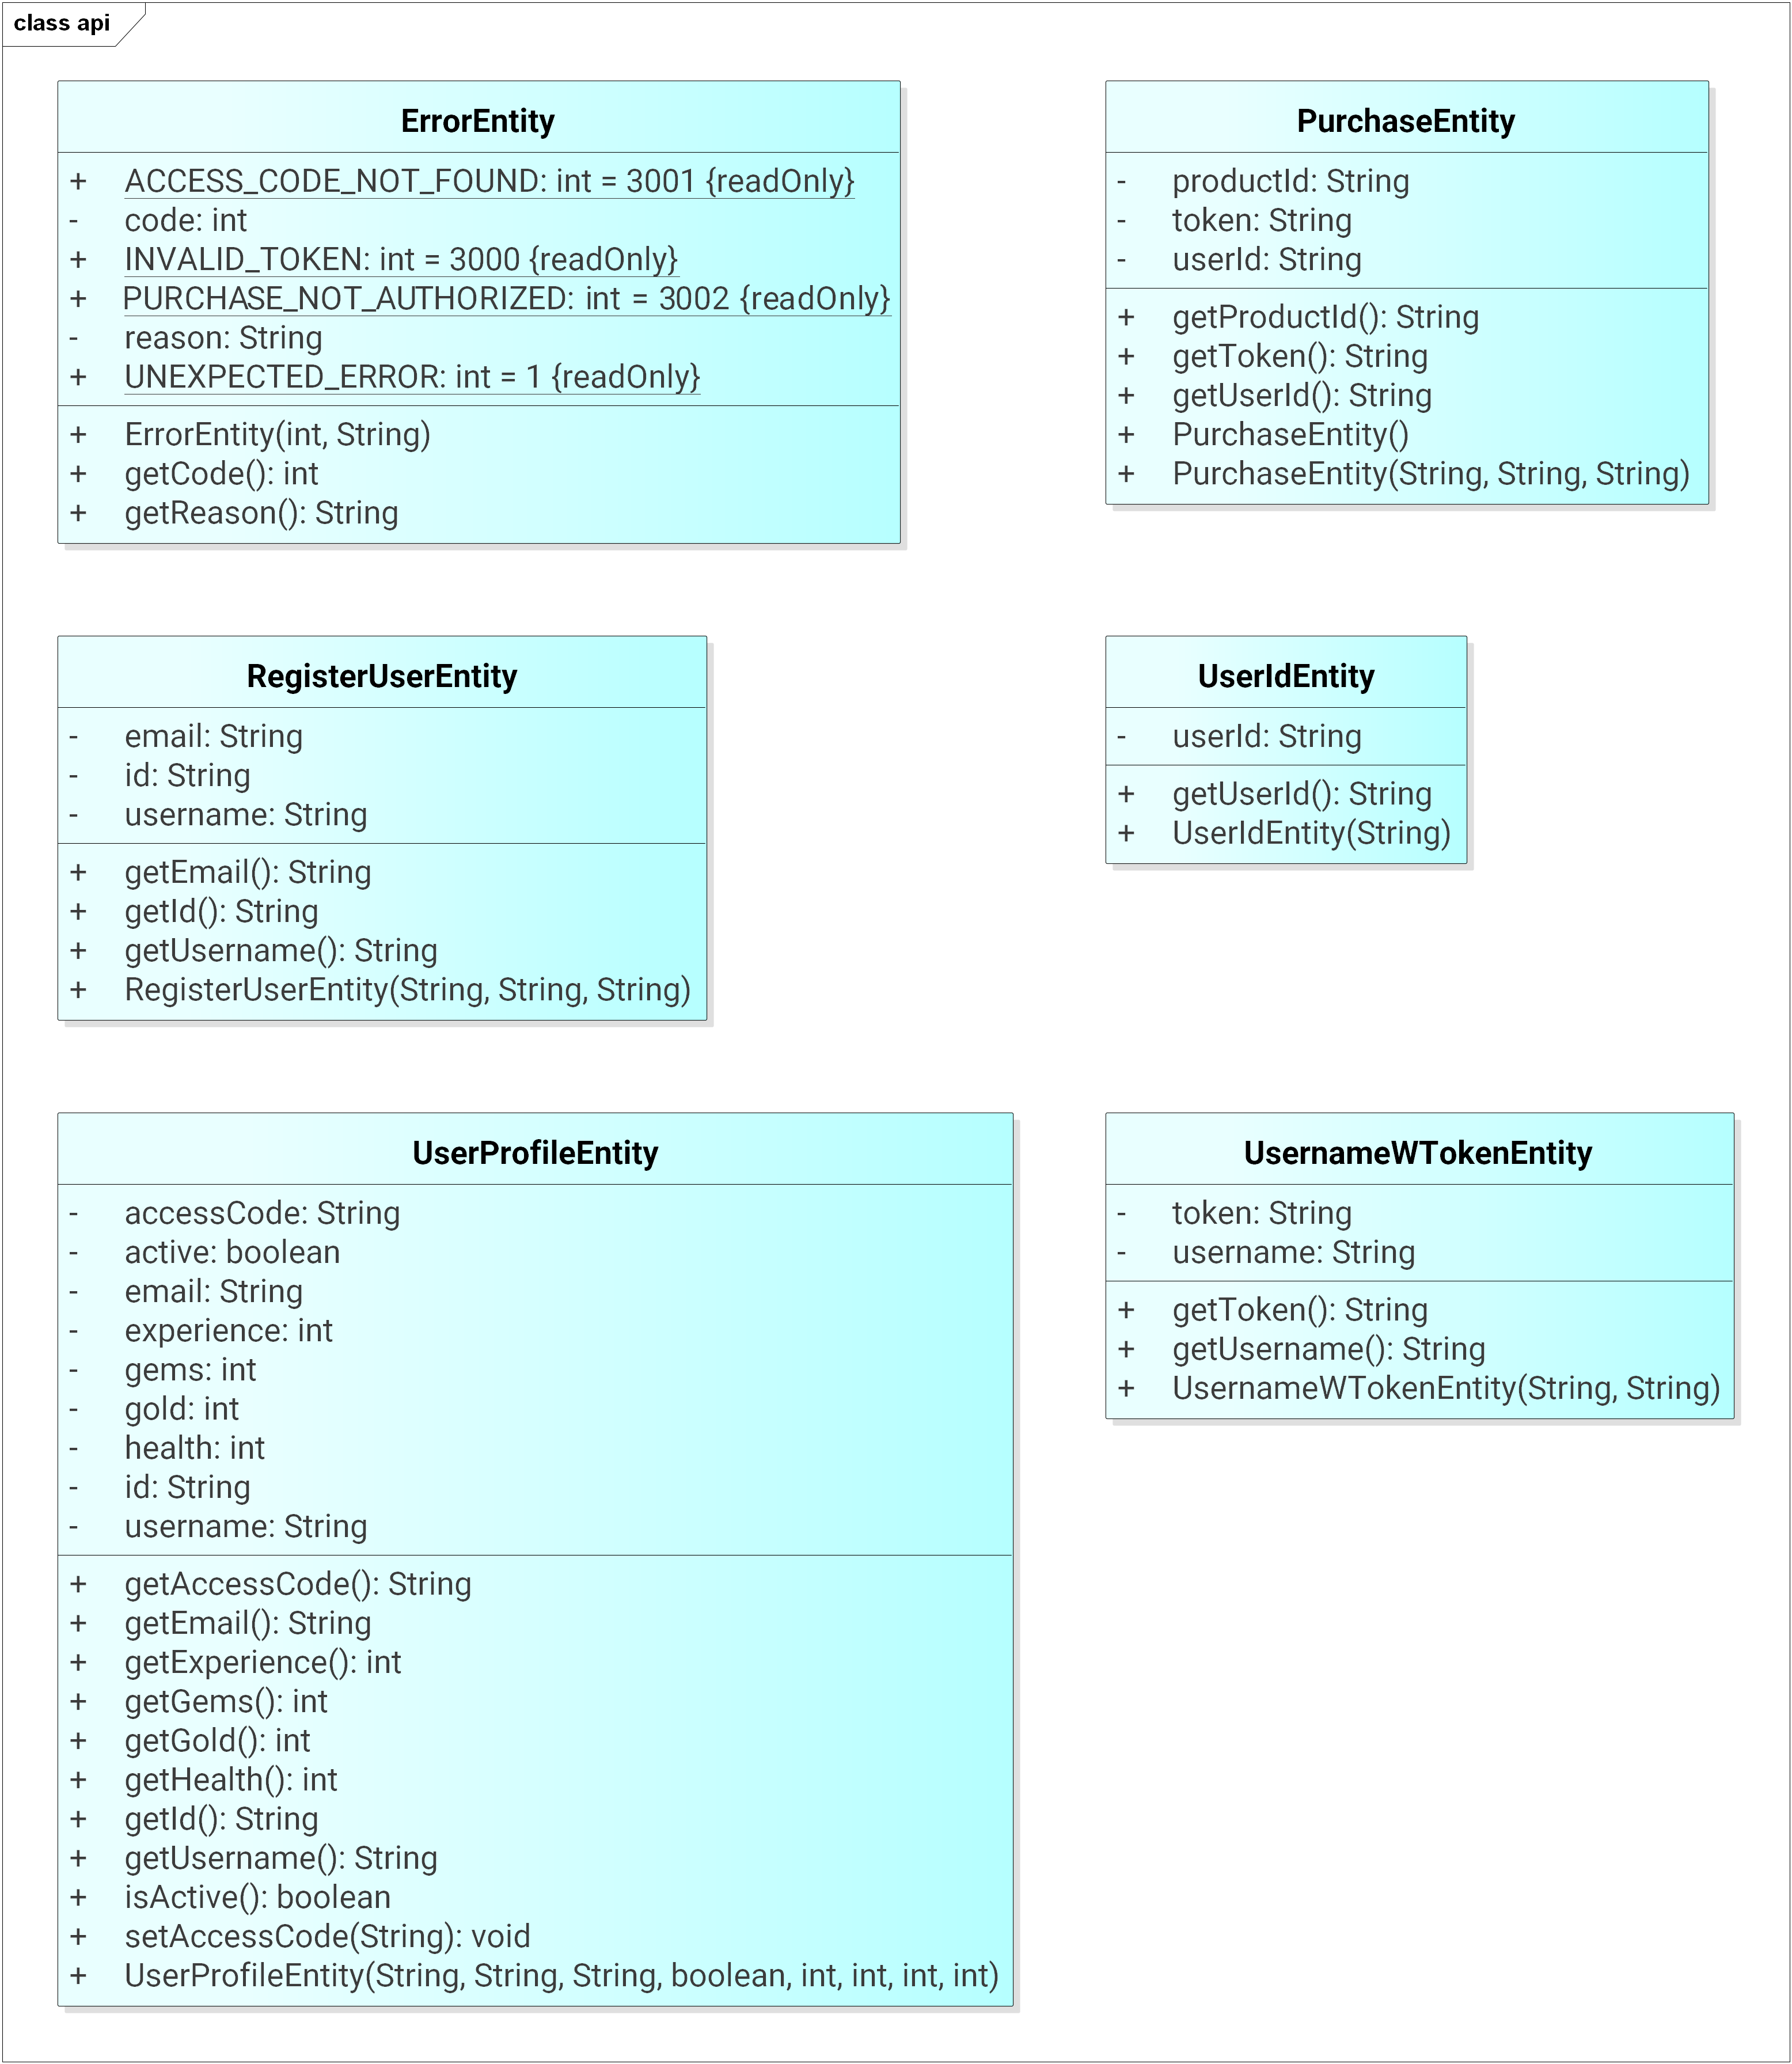
\includegraphics[width=\textwidth]{figures/classdiagrams/lsapi}
	\centering			
	\caption{Class diagram of package \textit{bachelors.login.api}}
\end{figure}

\begin{figure}[h]	
	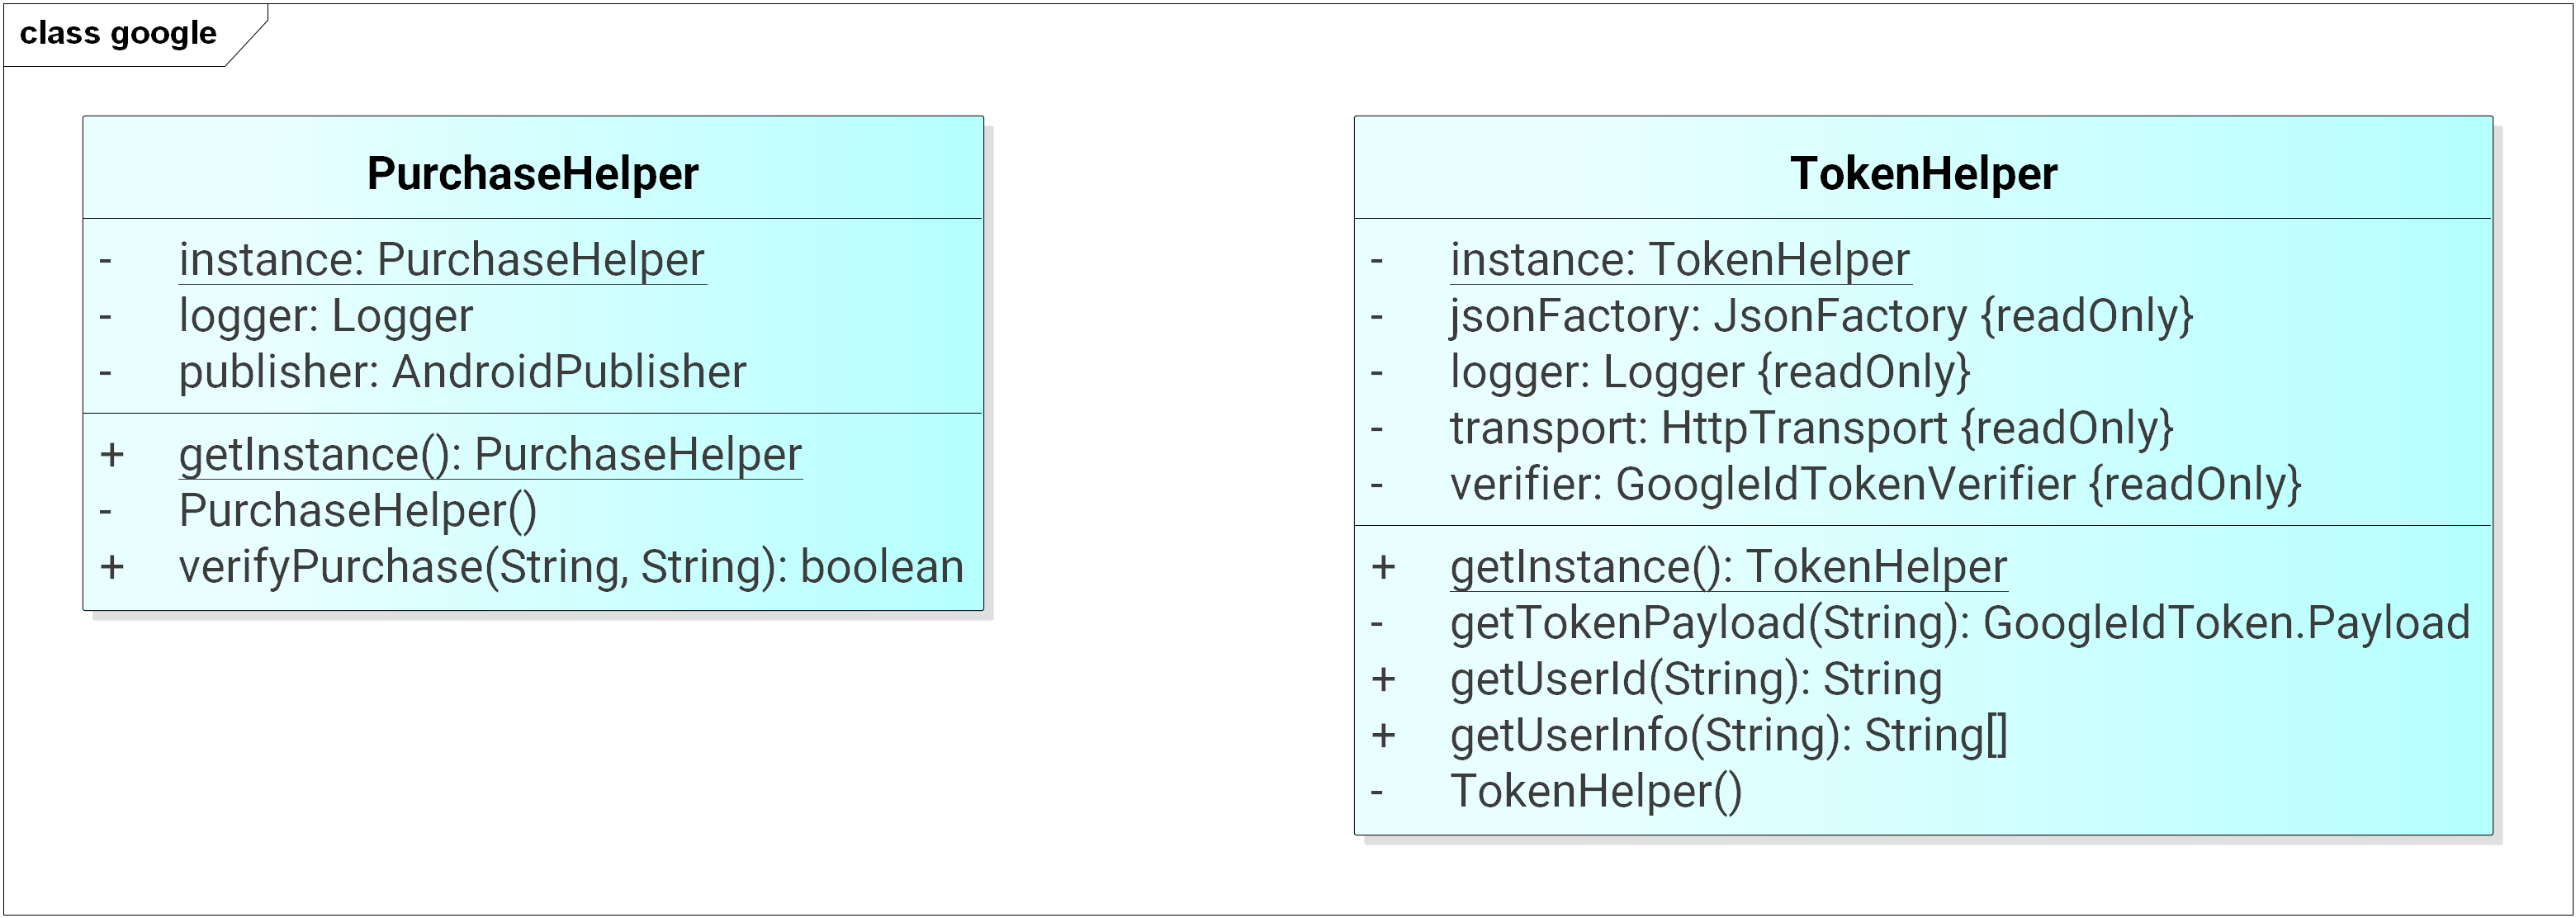
\includegraphics[width=\textwidth]{figures/classdiagrams/lsgoogle}
	\centering			
	\caption{Class diagram of package \textit{bachelors.login.google}}
\end{figure}

\begin{figure}[h]	
	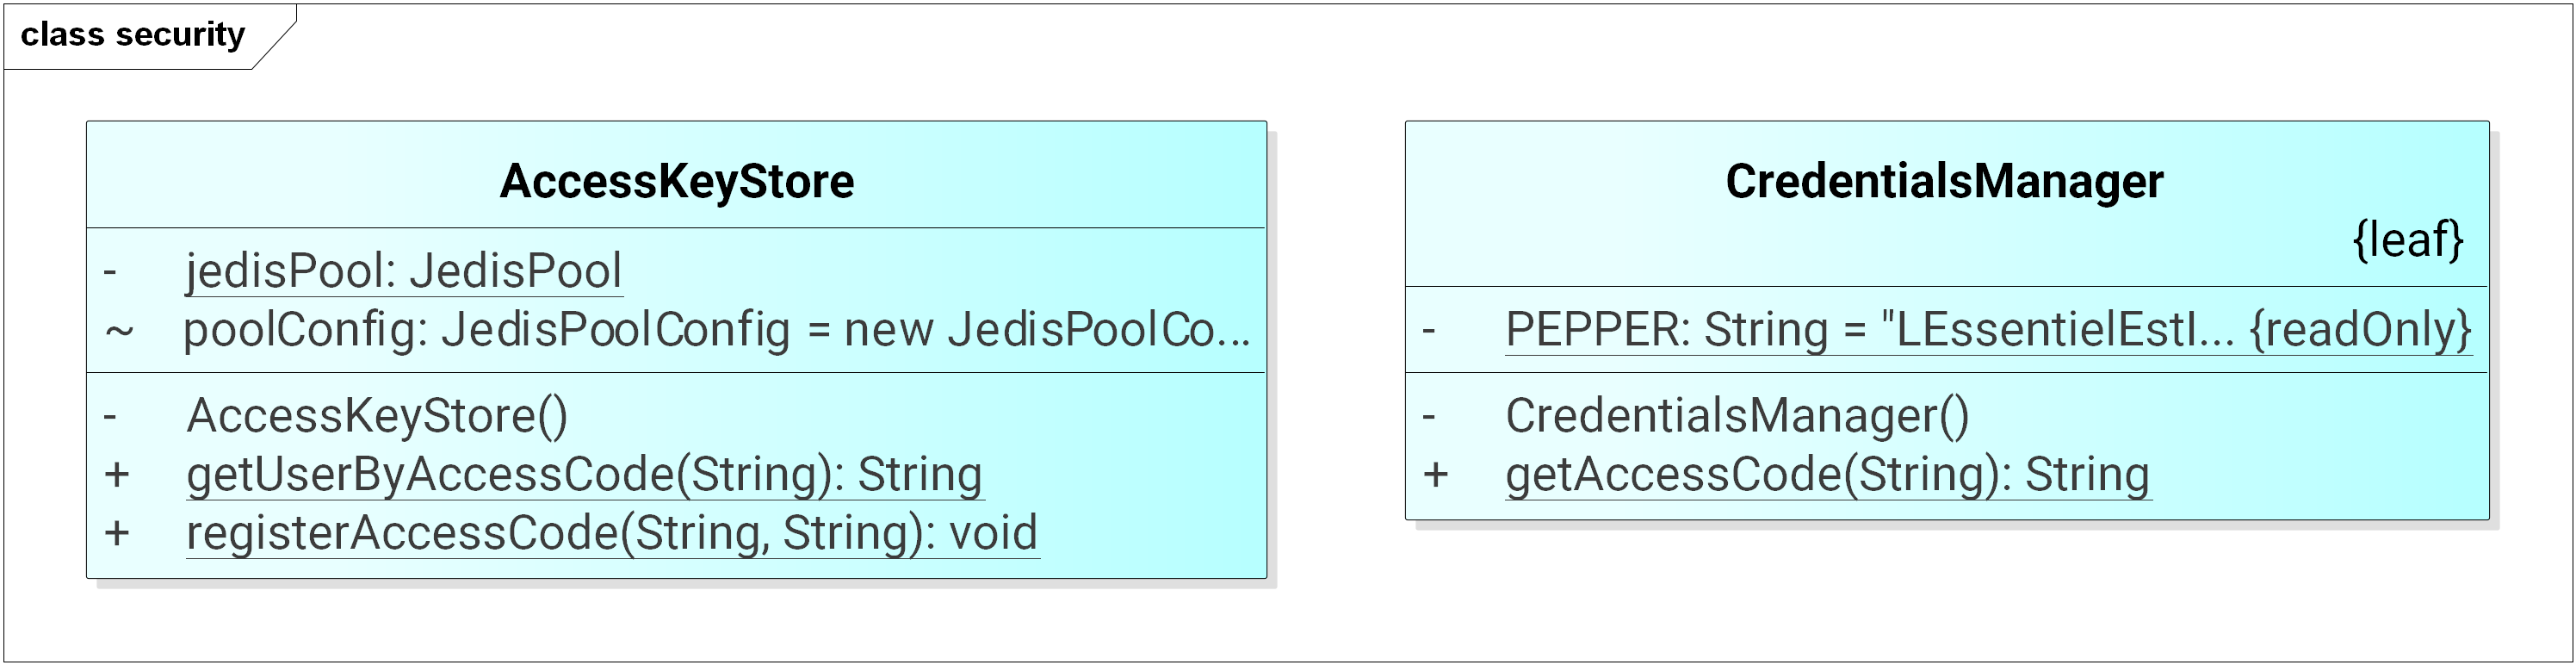
\includegraphics[width=\textwidth]{figures/classdiagrams/lssecurity}
	\centering			
	\caption{Class diagram of package \textit{bachelors.login.security}}
\end{figure}